\documentclass[12pt, letterpaper]{article}
\usepackage[titletoc,title]{appendix}
\usepackage{color}
\usepackage{booktabs}
\usepackage[usenames,dvipsnames,svgnames,table]{xcolor}
\definecolor{dark-red}{rgb}{0.75,0.10,0.10}
\definecolor{bluish}{rgb}{0.05,0.05,0.85}

\usepackage[margin=1in]{geometry}
\usepackage[linkcolor=blue,
			colorlinks=true,
			urlcolor=blue,
			pdfstartview={XYZ null null 1.00},
			pdfpagemode=UseNone,
			citecolor={bluish},
			pdftitle={partisan_gap}]{hyperref}

\usepackage[resetlabels,labeled]{multibib}
\newcites{SI}{SI References}
\usepackage{natbib}

\usepackage{float}

\usepackage{geometry}  % see geometry.pdf on how to lay out the page. There's lots.
\geometry{letterpaper} % This is 8.5x11 paper. Options are a4paper or a5paper or other...
\usepackage{graphicx}  % Handles inclusion of major graphics formats and allows use of
\usepackage{amsfonts,amssymb,amsbsy}
\usepackage{amsxtra}
\usepackage{verbatim}
\setcitestyle{round,semicolon,aysep={},yysep={;}}
\usepackage{setspace} % Permits line spacing control. Options are:
%\doublespacing
%\onehalfspace
\usepackage{sectsty}    % Permits control of section header styles
\usepackage{pdflscape}
\usepackage{fancyhdr}   % Permits header customization. See header section below.
\usepackage{url}        % Correctly formats URLs with the \url{} tag
\usepackage{fullpage}   %1-inch margins
\usepackage{multirow}
\usepackage{verbatim}
\usepackage{rotating}
\setlength{\parindent}{3em}

\usepackage[T1]{fontenc}
\usepackage[bitstream-charter]{mathdesign}

\usepackage{chngcntr}
\usepackage{longtable}
\usepackage{adjustbox}
\usepackage{dcolumn}

\usepackage[nameinlink, capitalize, noabbrev]{cleveref}

\def\citeapos#1{\citeauthor{#1}'s (\citeyear{#1})}

\makeatother

\usepackage{footmisc}
\setlength{\footnotesep}{\baselineskip}
\makeatother
\renewcommand{\footnotelayout}{\normalsize \doublespacing}


% Caption
\usepackage[hang, font=small,skip=0pt, labelfont={bf}]{caption}
%\captionsetup[subtable]{font=small,skip=0pt}
\usepackage{subcaption}

% tt font issues
% \renewcommand*{\ttdefault}{qcr}
\renewcommand{\ttdefault}{pcr}


\setcounter{page}{0}

\usepackage{lscape}
\renewcommand{\textfraction}{0}
\renewcommand{\topfraction}{0.95}
\renewcommand{\bottomfraction}{0.95}
\renewcommand{\floatpagefraction}{0.40}
\setcounter{totalnumber}{5}
\makeatletter
\providecommand\phantomcaption{\caption@refstepcounter\@captype}
\makeatother

\title{A Measurement Gap? Effect of the Survey Instrument on the Partisan Knowledge Gap}

\author{Lucas Shen\thanks{Email}, Gaurav Sood\thanks{Email}, and Daniel Weitzel\thanks{Asssitant Professor, Colorado State University, \href{mailto:daniel.weitzel@colostate.edu}{daniel.weitzel@colostate.edu}}}


\date{\today \thanks{Working paper, most recent version available at: \href{https://github.com/soodoku/partisan-gaps}{https://github.com/soodoku/partisan-gaps}}}

\begin{comment}

setwd(paste0(githubdir, "partisan-gaps/ms/"))
tools::texi2dvi("partisan_gap.tex", pdf = TRUE, clean = TRUE)
setwd(githubdir)

\end{comment}

\begin{document}
\maketitle
\thispagestyle{empty}

\begin{abstract}

\noindent Conventional wisdom suggests large, persistent gaps between partisans' stores of political knowledge, fanning concerns about democratic accountability. We reconsider the frequency and size of these ``partisan knowledge gaps,'' in  series of experiments. Manipulating frequently used survey items we demonstrate that survey design can inflate the partisan gap by YY\%. Our findings suggest that knowledge gaps---when they do exist---stem more from motivated responding than genuine differences in factual knowledge.

\end{abstract}

\vspace{.2in}

%{\bf Keywords:} Knowledge; Partisan Gap; Motivated Skepticism

\newpage

\doublespacing

The idea of a well-functioning representative democracy rests on the assumption of a more or less informed citizenry holding its representatives and political parties accountable for the successes and failures in office \citep{schattschneider-1960}. Partisan divisions raise concerns about this process of democratic accountability. In particular, research showing large differences in what partisans believe to be true about politically consequential things has cast a shadow on the prospect of democracy \citep{campbell1980american,bartels_2002,jerit2012partisan}.
% ``perceptual screen'' campbell1980american p. 133
If partisanship is in fact the pervasive force that perpetuates and reinforces how partisans see and understand the political world \citep[p. 138]{bartels_2002} serious normative implications about the functioning of democracy arise. A new line of research, however, suggests that a large fraction of the observed partisan difference in beliefs is an artifact of the survey response process \citep{bullocketal_2015,huber_yair_2018, prior2015you}. For instance, \cite{bullocketal_2015} find that nearly half the partisan gap in political knowledge is not a result of differences in beliefs but a result of expressive responding or partisan inference.

In this paper, we extend the investigation into the role of survey design in explaining partisan differences. We propose two theories of partisan gaps. The first argues that partisan gaps reflect actual differences in beliefs about the world. The second proposes that partisan gaps are, to a large part, artifacts of survey and questionnaire design. We report results from a new set of experiments that manipulate common features of frequently used survey items. The features we focus on plausibly encourage people to guess when they don't know or report attitudes instead of knowledge, and thereby encourage partisan inference causing inflated partisan gaps in knowledge. We also assess what difference items that not only assess knowledge but also confidence in that knowledge make on the prevelance and size of partisan gaps. Do these gaps persist if only responses that participants are confident in are coded as correct?
%more stringent way to code the answers---only coding responses that respondents are confident about as correct---makes to observed differences.
Across two experiments and YY items, we find that about YY\% of the knowledge differences between partisans are due to survey measures that encourage respondents to guess when they don't know. Across two other experiments, we find that features that encourage partisan inferences inflate the observed differences by KK\%. Lastly, we find that a coding scheme that only codes answers that respondents are confident in reduces partisan gaps by BB\% to LL\%. Our findings support the second theory of partisan knowledge gap formation. Current designs of survey items can encourage participants to not report confidently held knowledge but use partisan cues to express attitudes and opinions about the world.

\section*{Two Theories of Partisan Gaps}

Research has repeatedly shown that partisan gaps in political knowledge are wide and widespread \citep{bartels_2002, jerit2012partisan, lodgetaber_2013}. For instance, when Americans were quizzed at the end of Bill Clinton's first term in 1996 about whether the budget deficits increased, decreased, or remained the same, 39\% of Democrats correctly identified that the budget deficit had decreased, only 25\% of Republicans did the same \citep[280]{achen2016democracy}.
% Should we add a more recent example here?

There are two broad explanations for these gaps: The first is that partisan gaps on partisan consequential knowledge and misinformation items are a result of the fact that partisans know different things. The second theory is that partisans gaps are an artifact of the survey design.


% THIS IS THE SAME AS ABOVE
%\subsection*{Partisan Gaps in Knowledge}
%Research shows that partisan gaps in political knowledge are wide and widespread \citep{bartels_2002, jerit2012partisan, lodgetaber_2013}. For instance, when Americans were quizzed at the end of Bill Clinton's first term about whether the budget deficits increased, decreased, or remained the same during the last four years, while 39\% of Democrats correctly identified that the budget deficit had decreased, only 25\% of Republicans did the same \citep[280]{achen2016democracy}.

%There are two broad explanations for these gaps. The first is that partisan gaps on partisan consequential knowledge and misinformation items are a result of partisans knowing different things. The second theory is that partisan gaps are an artifact of the survey interview process.

\subsection*{Partisan Differences in Beliefs}
Partisan gaps in survey measures of political knowledge and misinformation may reflect \emph{actual differences} in what partisans believe to be true. These differences in beliefs may, in turn, stem from selective exposure to information---partisans being exposed to more congenial than uncongenial information \citep{peterson2021partisan}. Selective exposure to information can stem from a variety of processes. Even without partisans favoring congenial information, it could be that because of the kinds of people that partisans are, certain information is more readily available. For instance, African Americans, who overwhelmingly identify as Democrats, may be more exposed to negative consequences of economic downturns and may hence have different beliefs about economic conditions than Caucasians, a majority of whom identify as Republicans. Similarly, selective exposure may stem from different 'tastes' in politics. For instance, partisans of different stripes may be interested in different policies, politicians, etc. Taken thus, the gaps are similar to other types of knowledge gaps across groups---see research on gaps in gender \citep{dolan2011women, barabas2014question} and race \citep{abrajano2015reexamining}. Conventionally, however, partisan gaps are thought to stem from information avoidance---people find information that is dissonant to their worldview to be painful and work to avoid it  \citep[e.g.,][]{abelson1959modes,festinger1962theory}. % add Zaller1992 ?


peterson2021partisan

Whatever the cause, the effect of selective exposure is undoubtedly made worse by ``motivated skepticism'' \citep{taber2006, stroud2008media}. People are more skeptical of uncongenial than congenial information. Therefore, they may be more likely to follow up and do the due diligence to disprove uncongenial information. Or they may simply be more likely to distrust and ignore uncongenial information. People may also be less likely to remember uncongenial information.

To summarize, it is possible that the observed partisan gaps in political knowledge in survey research reflect actual differences in beliefs.

\subsection*{Artifact of Survey Design}
Partisan gaps on partisan consequential knowledge and misinformation items on surveys may be an \emph{artifact of questionnaire design}. 

The answers to survey questions about factual beliefs reflect a mixture of beliefs, inferences, cheating, expressive responding, and guesses. Inferences, cheating, and guessing cause structured error in our estimates, by inflating our estimates of how many people believe something. Our estimates of partisan gap in beliefs also suffer. Primarily, inferences with a partisan tint and expressive responding--responding to questions about beliefs to indicate partisan positions--inflate the estimates. On partisan consequential items---items where the right answer has implications about how good the party looks---inferences with a partisan tint are likely common. For instance, when partisans don't know the answer to a question, they likely use affect as a guide to infer the answer. For instance, when asked about what happened to the federal deficit during the Obama administration, Republicans, thinking Democrats cause bad things, may infer that deficits increased under Obama. Alternately, partisans may rely on stereotypical inference. Republicans may think of Democrats as generally indifferent to deficits, and hence may infer, without actually knowing, that it increased under Mr. Obama.

The extent to which survey responses are contaminated by responses other than strongly held beliefs depends on survey features. Surveys encourage respondents to respond 'expressively' by highlighting partisan motivations than accuracy motivations. \citep{Zaller1992} This explanation has attracted considerable research. Some of it shows that up to half of the partisan gaps are a result of expressive responding \citep{bullocketal_2015,huber_yair_2018, prior2015you}. (Though see \cite{berinsky_2017}.)

\subsection*{Empirical Implications of the Theories}

If partisan gaps are a result of actual differences, minor differences in question wording and response options stem should principally have little effect on the gap. On the other hand if the gaps are sensitive to question and response attributes, it suggests that some of the partisan gaps may not be founded in differences in beliefs. In particular, we contend that political surveys regularly include features that inflate partisan gaps to produce sensational results. Surveys regularly exclude don't know \citep{luskin2011don}, include guessing encouraging features such as providing background information and social proof in the stem that likely makes people think that they know something about the topic or give them extra information that they can use to guess the answer. Often enough, surveys also include partisan cues. And the scoring rules used by analysts doesn't disambiguate between respondents who are confident about their answers and those who aren't. Our hunch is that if you take out the inflationary features, the partisan gaps go down.

To test the conditionality of partisan knowledge gaps in survey data we fielded four surveys that test the effect different aspects of survey and question design can have on (partisan) response patterns. In studies 1 and 2, we used Amazon Mechanical Turk (MTurk) to ask participants a variety of knowledge questions in different designs. These items aim at examining how survey instructions, question wording, response options, and response design in the survey affect partisans to respond to questions in specific ways. In studies 3 and 4, we examine the role of question wording on response behavior in more detail by focusing on the effect that partisan-related auxilliary information can have on response patterns.

\section*{Impact of Don't Know, Neutral Information in the Question Stem, and Scoring Rules}

\subsection*{Data and Research Design}\label{sec:data}

Both surveys were fielded on Amazon's Mechanical Turk \citep{BerinskyHuberLenz2012} in the second quarter of 2017. In the first study, we randomly assigned 1,253 respondents to one of five conditions—Real World (RW), Iron Pyrite Standard (IP), Fewer Substantive Responses (FSR), 14k Gold Standard (14k), and the 24k Gold Standard (24k). In each condition respondents answered 9 misinformation items, ranging from citizenship and religion of Obama to whether global warming is happening or not. (The exact question wording for each of the items is presented in \cref{si:mturk}.) Respondents assigned to RW and IP saw a simple preface: ``Now here are some questions about what you may know about politics and public affairs,'' while in all the other conditions, they were reassured that it is ok to not know answers to these questions and to commit to not looking up answers or asking anyone and to mark don't know when they don’t know. (Again, see \cref{si:mturk} for the specific wording.)

In the second study, we randomly assigned 1,059 respondents to either closed-ended or confidence coding questions of four items. The topics and answer options of these questions were indentical to study 1 and included questions about the Affordable Care Act (2), the effect of greenhouse gases (1), and the consequences of then-president Trump's executive order on immigration(1). In the multiple choice version of the survey the participants received five options as answers, including a ``Don't Know'' option. In the confidence coding version of the survey respondents were asked to report the confidence with which they knew an item to be correct or incorrect. In this treatment the individuals were asked the same questions as in the multiple choice treatment and they had to report the confidence with which they considered each of the four statements that were answer options in the multiple choice questions to be correct or incorrect. The exact question wording for each of the items is presented in \cref{si:mturk2}.

\begin{itemize}

	\item Real World (RW): The RW condition reflects the real-world standards most closely--it does not feature a `Don't Know', it often features social proof about the incorrect answer, for instance, ``Some people believe Barack Obama was not born in the United States, but was born in another country'' on a question about where Mr. Obama was born, and some neutral information about the topic, like ``According to the Constitution, American presidents must be `natural born citizens''' on the birthplace question, that may encourage the ignorant to take a guess.
	
	\item No DK +  SP + GE: It never includes the 'Don't Know,' it always includes neutral information that encourages people to take a guess, and it also includes social proof about the incorrect answer.
	
	\item DK + SP + No GE: This condition adds a `Don't Know’ and removes from the question stem any neutral information that is likely to cause people to offer a substantive response when they don't know.
	
	\item DK + No SP + No GE: The best version of the multiple-choice question---no social proof, no guessing encouraging neutral wording, and a don't know---while maintaining commensurability with other items. 
	
	\item Confidence Scoring: Respondents rate the claim on a 0 to 10 scale going from `definitely false' to `definitely true.' The question is inspired by other attempts to take account of confidence in distinguishing misinformation from incorrect responses stemming from processes like inference, unlucky guessing, and such (see, for instance, \citep{pasek2015}).

\end{itemize}


\subsection*{Results}

\subsubsection*{Study 1}
We start by summarising the average partisan gap for each survey item and each treatment arm from the MTurk sample. \Cref{fig:partisangaps-mturk} shows the results. Each marker represents how much more congenial the responses of the Republicans are to the Democrats. In the RW treatment arm (first column), the Republicans are, on average, 30 percentage points more likely than the Democrats to have party-congenial responses. The subsequent four columns in \cref{fig:partisangaps-mturk} show that, while the estimated differences in party-congenial responses are precise (the narrow bars), the differences attenuated substantially depending on the treatment arms.

The attenuation is most pronounced when comparing the RW to the 24k arms (first vs. last columns). In the 24k arm, Republicans are, on average, only about 10 percentage points more likely to have party-congenial responses, a drop larger than 50 percent. \Cref{fig:partisangaps-mturk} therefore gives us the first indication that partisan gaps arise, at least in part, from questionnaire artefacts present in the different survey arms.

%\begin{table}[t] \centering \scriptsize \setlength\tabcolsep{0 pt} \setlength{\defaultaddspace}{0pt}
\caption{Unstandardized Partisan Gaps in Knowledge}
\label{tab:partisangaps-mturk}	
	\begin{adjustbox}{max width=\textwidth}
		\begin{tabular}{l*{15}{D{.}{.}{-1}}}	
			\toprule  
			& \multicolumn{3}{c}{RW} & \multicolumn{3}{c}{IPS} & \multicolumn{3}{c}{FSR} & \multicolumn{3}{c}{14k} & \multicolumn{3}{c}{24k} \\
			\cmidrule(lr){2-4} \cmidrule(r){5-7} \cmidrule(r){8-10} \cmidrule(r){11-13} \cmidrule(){14-16}                
			            & \multicolumn{1}{c}{Dem.}   & \multicolumn{1}{c}{Rep.} & \multicolumn{1}{c}{Gap} & \multicolumn{1}{c}{Dem.}   & \multicolumn{1}{c}{Rep.} & \multicolumn{1}{c}{Gap} & \multicolumn{1}{c}{Dem.}   & \multicolumn{1}{c}{Rep.} & \multicolumn{1}{c}{Gap} & \multicolumn{1}{c}{Dem.}   & \multicolumn{1}{c}{Rep.} & \multicolumn{1}{c}{Gap} & \multicolumn{1}{c}{Dem.}   & \multicolumn{1}{c}{Rep.} & \multicolumn{1}{c}{Gap} \\
			\cmidrule(lr){2-4} \cmidrule(lr){5-7} \cmidrule(lr){8-10} \cmidrule(lr){11-13} \cmidrule(l){14-16}    
			Obama birthplace    & 0.01       & 0.45       & 0.443    & 0.03       & 0.36       & 0.328    & 0.03       & 0.16       & 0.127    & 0.06       & 0.15       & 0.086      & 0.03       & 0.2        & 0.174    \\
			& {[}0.01{]} & {[}0.07{]} & {[}0.052{]} & {[}0.02{]} & {[}0.07{]} & {[}0.056{]} & {[}0.02{]} & {[}0.05{]} & {[}0.042{]} & {[}0.02{]} & {[}0.05{]} & {[}0.049{]} & {[}0.01{]} & {[}0.06{]} & {[}0.045{]} \\
			Obama religion      & 0.11       & 0.7        & 0.586    & 0.09       & 0.5        & 0.415    & 0.1        & 0.39       & 0.291    & 0.13       & 0.3        & 0.164     & 0.02       & 0.19       & 0.171    \\
			& {[}0.03{]} & {[}0.06{]} & {[}0.064{]} & {[}0.03{]} & {[}0.07{]} & {[}0.065{]} & {[}0.03{]} & {[}0.07{]} & {[}0.061{]} & {[}0.03{]} & {[}0.07{]} & {[}0.066{]} & {[}0.01{]} & {[}0.07{]} & {[}0.044{]} \\
			ACA illegal         & 0.21       & 0.68       & 0.465    & 0.17       & 0.66       & 0.490    & 0.1        & 0.34       & 0.238    & 0.17       & 0.43       & 0.256    & 0          & 0.15       & 0.147    \\
			& {[}0.04{]} & {[}0.06{]} & {[}0.074{]} & {[}0.04{]} & {[}0.07{]} & {[}0.073{]} & {[}0.03{]} & {[}0.06{]} & {[}0.060{]} & {[}0.04{]} & {[}0.07{]} & {[}0.072{]} & {[}0.00{]} & {[}0.06{]} & {[}0.044{]} \\
			ACA death panels    & 0.24       & 0.45       & 0.208    & 0.15       & 0.42       & 0.271    & 0.08       & 0.25       & 0.165    & 0.09       & 0.32       & 0.230    & 0.13       & 0.13       & 0.007       \\
			& {[}0.04{]} & {[}0.07{]} & {[}0.078{]} & {[}0.04{]} & {[}0.07{]} & {[}0.072{]} & {[}0.03{]} & {[}0.06{]} & {[}0.055{]} & {[}0.03{]} & {[}0.07{]} & {[}0.061{]} & {[}0.04{]} & {[}0.06{]} & {[}0.074{]} \\
			GW causes           & 0.09       & 0.66       & 0.569    & 0.06       & 0.62       & 0.556    & 0.13       & 0.48       & 0.355    & 0.06       & 0.57       & 0.512    & 0.01       & 0.26       & 0.248    \\
			& {[}0.03{]} & {[}0.07{]} & {[}0.063{]} & {[}0.03{]} & {[}0.07{]} & {[}0.061{]} & {[}0.03{]} & {[}0.07{]} & {[}0.064{]} & {[}0.02{]} & {[}0.07{]} & {[}0.059{]} & {[}0.01{]} & {[}0.07{]} & {[}0.043{]} \\
			GW scientists agree & 0.03       & 0.34       & 0.309    & 0.1        & 0.32       & 0.224    & 0.06       & 0.23       & 0.173    & 0.09       & 0.32       & 0.230    & 0.03       & 0.02       & -0.004      \\
			& {[}0.02{]} & {[}0.07{]} & {[}0.054{]} & {[}0.03{]} & {[}0.07{]} & {[}0.064{]} & {[}0.02{]} & {[}0.06{]} & {[}0.050{]} & {[}0.03{]} & {[}0.07{]} & {[}0.061{]} & {[}0.02{]} & {[}0.02{]} & {[}0.028{]} \\
			Voter fraud         & 0.16       & 0.66       & 0.497    & 0.12       & 0.8        & 0.683    & 0.14       & 0.36       & 0.213    & 0.1        & 0.26       & 0.157    & 0.04       & 0.18       & 0.142    \\
			& {[}0.04{]} & {[}0.07{]} & {[}0.070{]} & {[}0.03{]} & {[}0.06{]} & {[}0.062{]} & {[}0.03{]} & {[}0.06{]} & {[}0.065{]} & {[}0.03{]} & {[}0.06{]} & {[}0.060{]} & {[}0.02{]} & {[}0.06{]} & {[}0.046{]} \\
			MMR vaccine         & 0.12       & 0.17       & 0.047       & 0.05       & 0.2        & 0.147    & 0.06       & 0.16       & 0.101     & 0.05       & 0.15       & 0.095     & 0.01       & 0.02       & 0.014       \\
			& {[}0.03{]} & {[}0.05{]} & {[}0.059{]} & {[}0.02{]} & {[}0.06{]} & {[}0.052{]} & {[}0.02{]} & {[}0.05{]} & {[}0.047{]} & {[}0.02{]} & {[}0.05{]} & {[}0.047{]} & {[}0.01{]} & {[}0.02{]} & {[}0.021{]} \\
			Budget deficit      & 0.67       & 0.92       & 0.251    & 0.89       & 0.94       & 0.046       & 0.95       & 0.89       & -0.056      & 0.7        & 0.94       & 0.240    & 0.85       & 0.92       & 0.073       \\
			& {[}0.05{]} & {[}0.04{]} & {[}0.070{]} & {[}0.03{]} & {[}0.03{]} & {[}0.050{]} & {[}0.02{]} & {[}0.04{]} & {[}0.041{]} & {[}0.04{]} & {[}0.04{]} & {[}0.071{]} & {[}0.04{]} & {[}0.04{]} & {[}0.065{]} \\
			Average             & 0.12       & 0.49       & 0.375    & 0.09       & 0.44       & 0.347    & 0.08       & 0.29       & 0.207    & 0.09       & 0.32       & 0.225    & 0.03       & 0.13       & 0.099    \\
			& {[}0.02{]} & {[}0.03{]} & {[}0.030{]} & {[}0.02{]} & {[}0.04{]} & {[}0.036{]} & {[}0.02{]} & {[}0.03{]} & {[}0.032{]} & {[}0.02{]} & {[}0.03{]} & {[}0.033{]} & {[}0.01{]} & {[}0.03{]} & {[}0.025{]}\\
			\bottomrule                    
		\end{tabular}
	\end{adjustbox}
\caption*{\scriptsize Difference in partisan gaps in knowledge (Republican - Democrats) for each of the nine questions in the MTurk sample and for the average difference in knowledge gap over all nine questions. Standard errors in brackets.}
\end{table}

\begin{center}
	\begin{figure}[t]
		\centering
		\caption{Partisan Gap by Treatment Arm (MTurk)}
		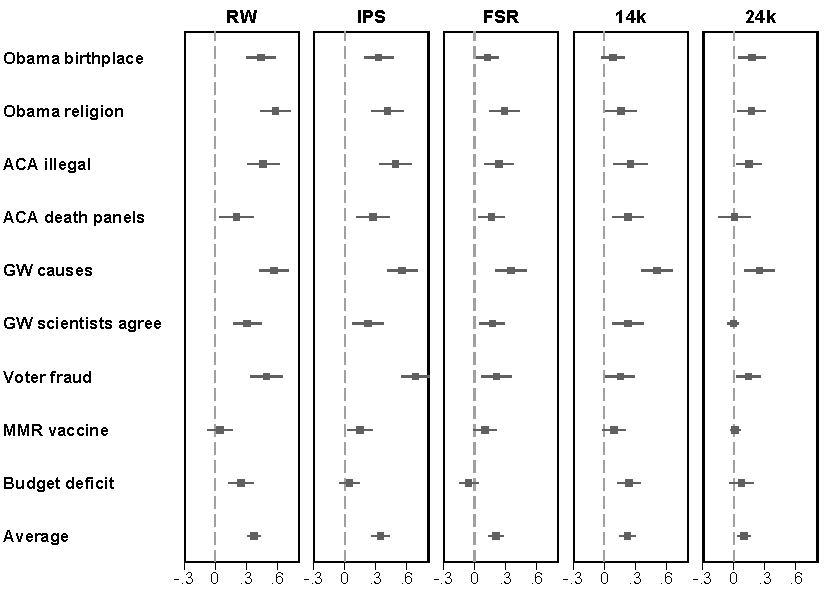
\includegraphics[width=\textwidth]{../figs/partisan-gap-by-item-arm.pdf}
		\label{fig:partisangaps-mturk}
		\caption*{\footnotesize 
			Each point is the estimated gap between Republicans and Democrats for how congenial their responses are to their own party.
			Columns indicate the five different treatment arms described in \nameref{sec:data}. Rows indicate the nine individual survey items described in \cref{si:mturk} plus their average.
			Each point is the estimated $\beta$ from estimating $1\{party\text{-}congenial\, response\}_i = \alpha + \beta Rep_i + \varepsilon_i$ for each of items and each of the five arms.			
			Horizontal bars are 95\% confidence intervals constructed from robust standard errors.
		}
	\end{figure}
\end{center}

\begin{center}
	\begin{figure}[t]
		\centering
		\caption{Partisan Gaps in Knowledge in different question designs}
		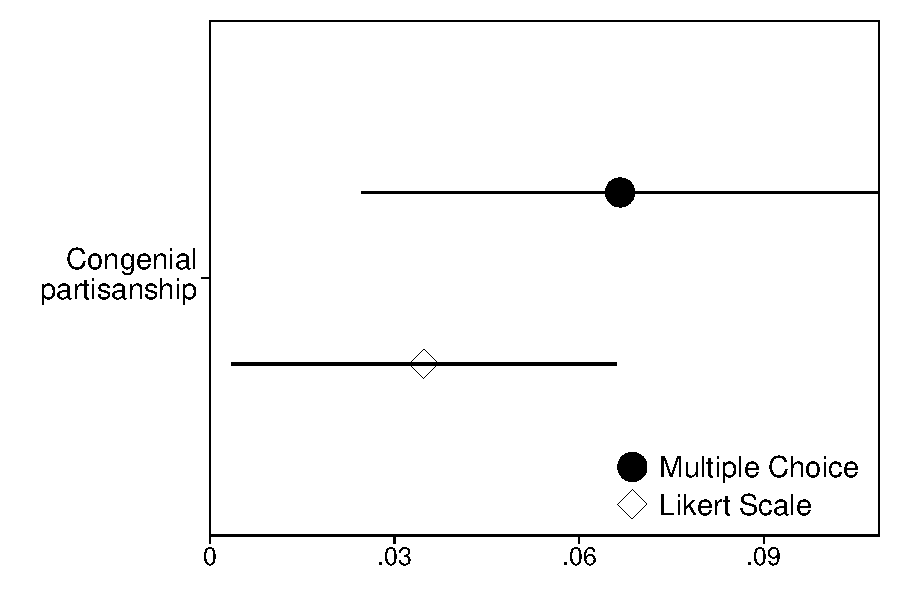
\includegraphics[width=.6\textwidth]{../figs/mturk-hk-MC-LIKERT.pdf}
		\label{fig:xxx}
		\caption*{\footnotesize 
		}
	\end{figure}
\end{center}

\begin{table}
   \caption{Partisan Gaps in Knowledge in different question designs}
   \label{tab:mturk_hk}
\begin{center}
 \begin{tabular}{l c c}
\hline
   & IMC     & CCD \\
   & Multiple Choice & Likert Scale \\
\hline
Congenial      & $0.07^{*}$      & $0.03^{*}$      \\
               & $ [0.02; 0.11]$ & $ [0.00; 0.07]$ \\
(Intercept)    & $0.19^{*}$      & $0.08^{*}$      \\
               & $ [0.15; 0.24]$ & $ [0.05; 0.12]$ \\
\hline
R$^2$          & $0.24$          & $0.25$          \\
Survey item FE & Yes             & Yes             \\
N Clusters     & $480$           & $422$           \\
Num. obs.      & $1920$          & $1688$          \\
\hline
\multicolumn{3}{l}{\scriptsize{$^*$ Null hypothesis value outside the confidence interval.}}
%	\caption*{\scriptsize{All models are linear probability models where the dependent variable indicates whether the response to a survey item is correct. The independent variable indicates whether the partisanship of the respondent is congenial with the content of the questions. The multiple choice model includes four items. Each of these items had four substantive response options with one correct option. All multiple choice questions included ``Don't know''. The Likert Scale items included the same questions as the Multiple Choice items. Here the four substantive questions were presented to the respondents and they were asked to rate on a scale from 0-10 how true each statement is. Answers were coded as correct for individuals that indicated 10 for the correct statement. Results are robust to a specification that codes greater than 7 as correct.  All models include survey item fixed effects. Standard errors are clustered at the respondent level.}}
  \end{tabular}
\end{center}
\end{table}


\subsubsection*{Study 2}

We formalize the above observation as follows. We regress the dependent variable, an indicator of whether the response is party-congenial, on the interaction of partisanship and the treatment arm:
\begin{equation}\label{eq:partisangap-mturk}
y_{ijk} = \alpha + \beta (Rep)_i + \gamma (Arm)_k + \delta_k (Rep_i \times Arm_k) + (survey \; item)_j + \varepsilon_{ijk}
\end{equation}
for respondent $i$, survey item $j$, and treatment arm $k$. $\beta$ is the difference in partisan knowledge gaps, which corresponds to \cref{fig:partisangaps-mturk}. A positive estimate suggests that Republicans are more likely than Democrats to have a party-congenial response. We focus on the $\delta$'s, which capture how the different treatment arms affect observed partisan knowledge gaps (difference between columns in \cref{fig:partisangaps-mturk}). The baseline treatment arm is always RW, so $\delta$ captures how the four treatment arms---having the same questions with different questionnaire artefacts---mediates partisan knowledge gaps.
We include the survey item fixed effects to allow each item to elicit some constant amount of partisan gap, if any, from the respondents. Standard errors are clustered at the respondent level.

\begin{figure}[!t]
	\centering
	\caption{Partisan Gap by Treatment Arm: MTurk}
	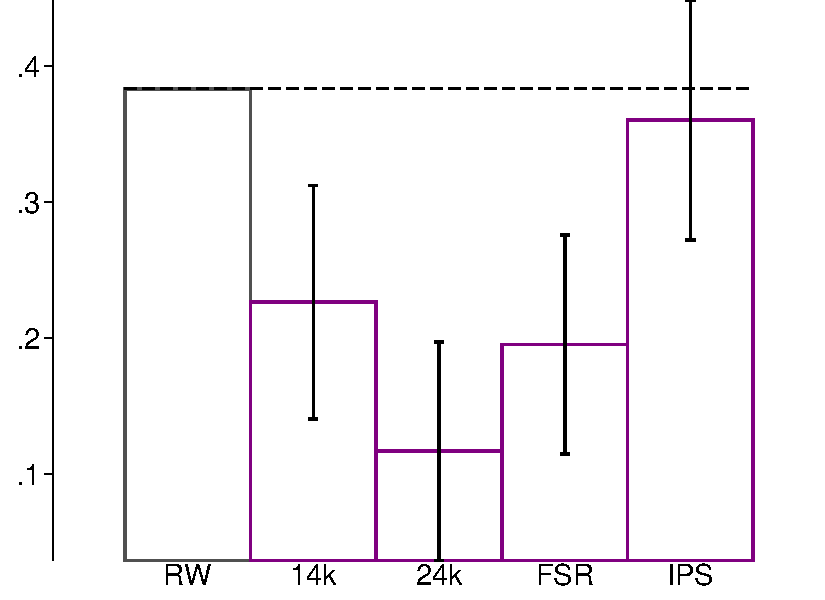
\includegraphics[width=.55\textwidth]{../figs/mturk-pgag-surveyarms.pdf}
	\label{fig:partisangaps-mturk-reg}
	\caption*{\footnotesize 
		Difference between bars indicates the predicted partisan gap by the treatment arms. 
		Bars reconstructed from the interactions of the Republican indicator with the treatment arms as reported in column (3) of \cref{tab:partisangaps-mturk}.
		The baseline arm is RW.
		Capped vertical bars are 95\% confidence intervals.
	}
\end{figure}


\begin{table}[t] \centering \small \setlength\tabcolsep{0 pt} \setlength{\defaultaddspace}{0pt}
	\def\sym#1{\ifmmode^{#1}\else\(^{#1}\)\fi}
	\caption{Partisan Knowledge Gaps: MTurk}
	\label{tab:partisangaps-mturk}
	\begin{adjustbox}{max width=\textwidth}
		\begin{tabular}{l*{6}{D{.}{.}{-1}}}
			\toprule
			% https://tex.stackexchange.com/questions/567985/problems-with-inputtable-tex-hline-after-2020-fall-latex-release
			\input ../tabs/mturk-reg-table-fragment.tex
			\bottomrule
		\end{tabular}
	\end{adjustbox}
	\caption*{\footnotesize All models are linear probability models where the dependent variable indicates whether the response to a survey item is congenial to party affiliation. Demographic controls include age cohort, gender, education level (college degree, high school, no high school, post-graduate, and some college), and race (Hispanic, Asian, Black, White, Others). All models include the nine survey item fixed effects. Standard errors are clustered at the respondent level. Significance levels: + 0.1 * 0.05 ** 0.01 *** 0.001.}
\end{table}


\cref{tab:partisangaps-mturk} reports the results from estimating \cref{eq:partisangap-mturk}. Column (1) includes just the Republican variable, which is significant and consistent with conventional wisdom about gaps in partisan knowledge \citep[e.g.][]{bullocketal_2015, pew2018disagree}.
Column (2) includes only the treatment arms, and three of them elicit differences in partisan gaps that are statistically different from the baseline RW arm. While the treatment arm estimates are not as large as the Republican variable in column (1), it is still substantial evidence of how variable the estimated knowledge gap can be in the presence of questionnaire artefacts.

Moreover, it is variable in a way that is independent of partisanship. Without accounting for partisanship, for instance, the average respondent assigned to the 24k arm is 17 percentage points less likely to give a party-congenial response than the RW arm ($p<0.001$). This gap is approximately two-thirds of the estimated effect of partisanship on the partisan knowledge gap.

In column (3) of \cref{tab:partisangaps-mturk}, we include the interaction of partisanship and treatment arms. Now the Republican variable captures the partisan gap in the RW arm (corresponding to column (1) of \cref{fig:baltest-24k-rw}). The Republican and treatment arms interactions reveal the extent to which partisan knowledge gap changes across the different treatment arms. 

\cref{fig:partisangaps-mturk-reg} shows the estimates in absolute terms. For the FSR interaction term, just adding a `Don't Know' response option reduces the estimated partisan knowledge gap by half ($p<0.001$).
The largest reduction is 71 percent ($p<0.001$), which comes from the 24k arm. This arm allows respondents to rate their responses on a 0 to 10 scale from `definitely false' to `definitely true' instead of a false and true option. Including self-reported characteristics of respondents in columns (4)--(6) does not change this conclusion. Overall, the MTurk sample reveals that measured partisan knowledge gaps are highly sensitive to different questionnaire artefacts in the same questions.


\section*{Impact of Partisan Cues on Partisan Gaps}\label{subsec:partisan-cues}
The aim of the study is to present experimental evidence about effect of partisan cues in the question stem on responses by partisans. For the purpose of the study, we examine closed-ended items asking about policy-relevant facts or objective performance, particularly those items stirring affective consistency, stereotyping, or both.  In the first case, items whose correct response option one side or the other would like to disbelieve, or at least one of whose incorrect response options one side or the other would like to believe, or both; in the second case items whose correct response option defies stereotype, or at least one of whose incorrect response options conforms to stereotype, or both.  

For exploring the research question, we exploit two datasets---a national survey conducted by YouGov, and a telephone survey of a random sample of adults in Texas. The YouGov survey interviewed 2000 respondents between July 10th and 12th, 2012.  In Texas, a total of 1003 interviews were conducted between September 10th and 21st, 2012. 

In the YouGov survey, respondents were randomly assigned to factual questions with either a Republican or Democratic cue in the stem. In a question about whether ``since 2010 midterm elections, the unemployment rate [had] gone up, down, or remained the same, or couldn't you say?'', we inserted either the phrase “when Republicans regained control of the U.S. Congress'' or ``when Democrats retained control of the Senate” right after the first phrase. We employed a similar manipulation for the question on budget deficit, asking how the budget deficit had fared “since the 2010 midterm elections, when Republicans regained control of the U.S. Congress (or ``when Democrats retained control of the Senate''), has the budget deficit gone up, gone down, remained the same, or couldn't you say?''

In the Texas survey, we added another condition to the above design – no partisan cue in the stem. So a third of the respondents were assigned to a question that simply read, ``since the 2010 midterm elections, has the unemployment rate gone up, gone down, or remained the same?  Or couldn’t you say?'' For the second question we changed our design to – no partisan cue, Democratic cue, and Democratic cue plus the following introduction “based on what you have heard”. The question read, ``since January 2009, have federal taxes increased, decreased, or remained the same or couldn’t you say?.'' The second version gave respondents a Democratic cue by changing the initial part of the sentence; the question now read, “Since Barack Obama took office\ldots''  The third version prepended a cue designed to encourage guessing to the second version; the version read, “Based on what you have heard, since Barack Obama took office, \ldots''


\subsection*{Results: Partisan Knowledge Gaps with Partisan Cues (YouGov)}
\begin{figure}[t]
	\caption{Partisan Knowledge Gaps with Partisan Cues: YouGov Survey}	
	\centering
	\begin{subfigure}{.495\textwidth}\centering
		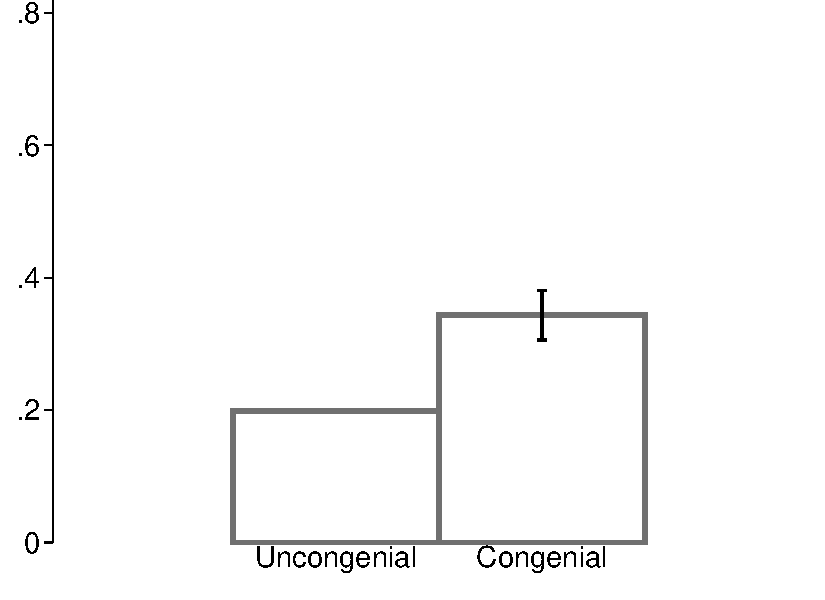
\includegraphics[width=\textwidth]{../figs/yougov-unemp-congenialcue.pdf}
		\caption{Unemployment}
	\end{subfigure}
	\hfil
	\begin{subfigure}{.495\textwidth}\centering
		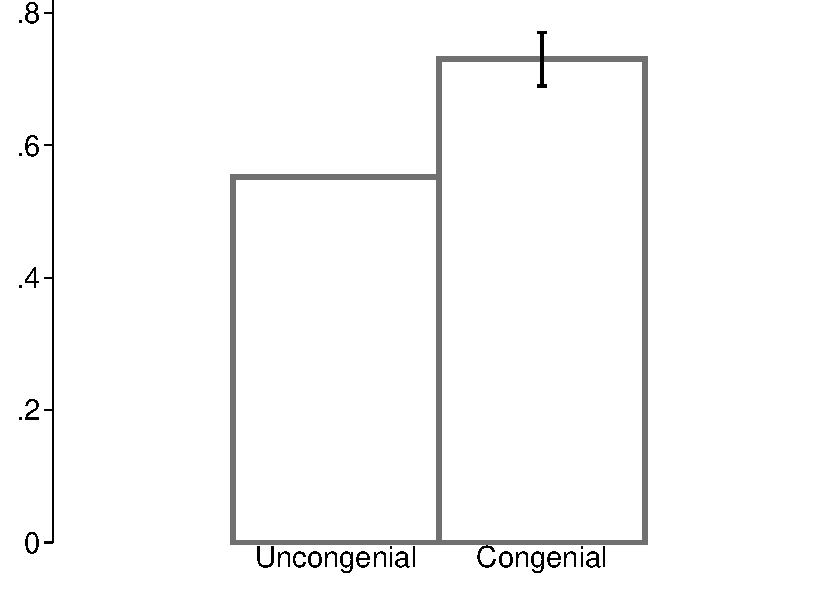
\includegraphics[width=\textwidth]{../figs/yougov-deficit-congenialcue.pdf}
		\caption{Budget deficit}
	\end{subfigure}	
	\caption*{\footnotesize Bars indicate the predicted percent of responses saying that unemployment or the budget deficit have gone up (correct responses) as reported in \cref{tab:partisangaps-yougov} (columns (1) and (4)).  
		Capped vertical bars indicate 95\% confidence intervals.
	}
	\label{fig:yougov-reg}
\end{figure}

We start with the YouGov survey to provide experimental evidence that cues in survey questions can affect responses to questions about policy-relevant and objectively verifiable facts. This survey includes questions about changes in unemployment and the budget deficit since the 2010 midterm elections, with manipulated partisan cues in the stem. 

Using the YouGov survey responses, we estimate
\begin{equation}\label{eq:pgap-yougov}
\text{correct response}_{i} = \alpha + \beta (congenial \; cue)_i  +\varepsilon_{i},
\end{equation}
where the dependent variable is the indicator for whether the response to the question is correct.
As discussed above in \cref{subsec:partisan-cues}, we model the correct response rate as dependent on whether the cue presented to individuals is congenial to responding correctly. Specifically, the congenial cue indicator is coded as one when a Democrat receives a question stem with the cue ``when Republicans gained control of the US congress.'' This cue manipulates Democrats into blaming the Republicans by suggesting that unemployment has gone up, which is the correct response. The reverse happens for Republicans. The congenial cue for Republicans is coded as one when they receive the cue ``When Democrats retained control of the Senate.''

\begin{table}[t] \centering \normalsize \setlength\tabcolsep{0 pt} \setlength{\defaultaddspace}{0pt}
	\def\sym#1{\ifmmode^{#1}\else\(^{#1}\)\fi}
	\caption{Partisan Knowledge Gaps with Partisan Cues: YouGov}
	\label{tab:partisangaps-yougov}
	\begin{adjustbox}{max width=\textwidth}
		\begin{tabular}{@{\hspace{0\tabcolsep}}l*{6}{D{.}{.}{-1}}@{\hspace{0\tabcolsep}}}
			\toprule
			% https://tex.stackexchange.com/questions/567985/problems-with-inputtable-tex-hline-after-2020-fall-latex-release
			&\multicolumn{3}{c}{Unemployment has gone up}&\multicolumn{3}{c}{Deficit has gone up}\\
			\cmidrule(lr){2-4}\cmidrule(l){5-7} 
			\input ../tabs/yougov-reg-table-fragment.tex
			\bottomrule
		\end{tabular}
	\end{adjustbox}
	\caption*{\footnotesize Dependent variables are indicators for whether the individual responded that unemployment or the budget deficit had gone up since the 2010 midterm elections (which are the correct responses).
		Congenial cue is an indicator of whether the question stem includes the cue towards getting the correct response. For Democrats, this is when the question stem includes the cue ``when Republicans gained control of the US Congress.''
		For Republicans, this is when the question stem includes the cue ``when Democrats retained control of the Senate.''
		Demographic controls include age cohort, gender, education level, marital status, employment status, news interest, family income, and race. Standard errors are heteroskedasticity-robust. 
		All models are linear probability models. 
		Significance levels: + 0.1 * 0.05 ** 0.01 *** 0.001.}
\end{table}
Panel (a) of \cref{fig:yougov-reg} shows that, by manipulating the partisan cue that respondents receive, the probability of getting the correct response for the unemployment question differs by 14 percentage points ($p < 0.001$, reported in \cref{tab:partisangaps-yougov}).

Panel (b) of \cref{fig:yougov-reg} shows that this systematic difference is not unique to the unemployment question. We reestimate \cref{eq:pgap-yougov} where the dependent variable is getting the correct response that the budget deficit has gone up. When the individuals get a congenial cue, they are 18 percentage points more likely to get the correct response ($p<0.001$).
Presumably, we observe this congenial cue effect because the question stem holds the other party responsible for the increase in unemployment and deficit, which are both undesirable.\footnote{\cref{fig:yougov-reg-by-partisanship} show that there is some heterogeneity in how the congenial cue affects Republicans as opposed to Democrats. However, the effect is not unique to either party since partisans of both types are more likely to get the correct response when randomly assigned the congenial cue.}

\subsection*{Results: Partisan Knowledge Gaps with Partisan Cues (Texas Lyceum)}
\begin{figure}[!t]
	\centering
	\caption{Partisan Gap by Treatment Arm: Texas Lyceum, Unemployment}
	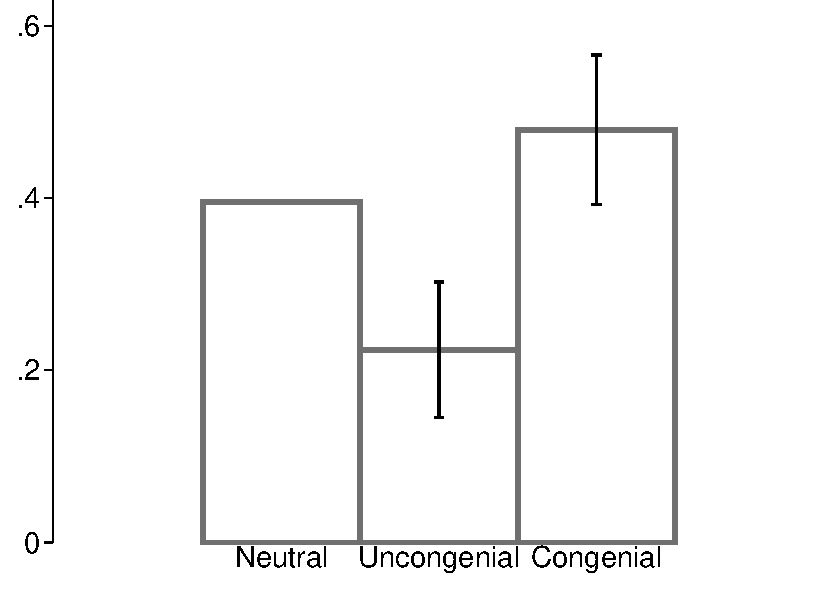
\includegraphics[width=.55\textwidth]{../figs/texas-unemp-congenialcue.pdf}
	\label{fig:partisangaps-texas-unemp}
	\caption*{\footnotesize 
		Bars indicate the predicted percent of responses saying that unemployment has gone up (correct response) as reported in column (1) of \cref{tab:partisangaps-texas-unemp}.  
		Capped vertical bars indicate 95\% confidence intervals.
	}
\end{figure}

We further supplement our results with the Texas Lyceum survey, which includes a third cue: a neutral cue. For the question about unemployment in this survey, in addition to congenial and uncongenial cues, individuals can also be randomly assigned a neutral cue where the additional question stem assigning blame to a party is absent, giving us a total of three groups: (i) no cue, (ii) congenial cue, and (iii) uncongenial cue.

\cref{fig:partisangaps-texas-unemp} shows that our results above still hold when we include a neutral cue. Compared to individuals who received a neutral cue, individuals who receive an uncongenial cue are 17 percentage points less likely to get the correct answer that unemployment has gone up ($p<0.001$). Individuals who receive a congenial cue are 8 percentage points more likely to get the correct answer ($p<0.1$). These results are tabulated in \cref{tab:partisangaps-texas-unemp}.

\begin{table}[t] \centering \normalsize \setlength\tabcolsep{6 pt} \setlength{\defaultaddspace}{0pt}
	\def\sym#1{\ifmmode^{#1}\else\(^{#1}\)\fi}
	\caption{Partisan Knowledge Gaps with Partisan Cues: Texas Lyceum, Unemployment}
	\label{tab:partisangaps-texas-unemp}
	\begin{adjustbox}{max width=\textwidth}
		\begin{tabular}{@{\hspace{0\tabcolsep}}l*{3}{D{.}{.}{-1}}@{\hspace{0\tabcolsep}}}
			\toprule
			% https://tex.stackexchange.com/questions/567985/problems-with-inputtable-tex-hline-after-2020-fall-latex-release
			&\multicolumn{3}{c}{Unemployment has gone up}\\
			\cmidrule(l){2-4}
			\input ../tabs/texas-unemp-reg-table-fragment.tex
			\bottomrule
		\end{tabular}
	\end{adjustbox}
	\caption*{\footnotesize Dependent variable is an indicator for whether the individual responded that unemployment has gone up since the 2010 midterm elections (which is the correct response).
		Congenial cue is an indicator of whether the question stem includes the cue towards getting the correct response. 
		For Democrats, this is when the question stem includes the cue ``when Republicans regained control of the US Congress.''
		For Republicans, this is when the question stem includes the cue ``when the Democrats retained control of the Senate.''
		Demographic controls include age cohort, gender, education level, marital status, number of children, children school enrollment, family income, religion, liberalism/conservatism, and race. Standard errors are heteroskedasticity-robust. 
		All models are linear probability models. 
		Significance levels: + 0.1 * 0.05 ** 0.01 *** 0.001.}
\end{table}


\begin{table}[t] \centering \normalsize \setlength\tabcolsep{6 pt} \setlength{\defaultaddspace}{0pt}
	\def\sym#1{\ifmmode^{#1}\else\(^{#1}\)\fi}
	\caption{Partisan Knowledge Gaps with Partisan Cues: Texas Lyceum, Federal Taxes}
	\label{tab:partisangaps-texas-fedtax}
	\begin{adjustbox}{max width=\textwidth}
		\begin{tabular}{@{\hspace{0\tabcolsep}}l*{4}{D{.}{.}{-1}}@{\hspace{0\tabcolsep}}}
			\toprule
			% https://tex.stackexchange.com/questions/567985/problems-with-inputtable-tex-hline-after-2020-fall-latex-release
			&\multicolumn{2}{c}{Responded ``Gone up''}&\multicolumn{2}{c}{Responded ``Don't Know''}\\
			\cmidrule(lr){2-3}\cmidrule(l){4-5} 
			\input ../tabs/texas-fedtax-reg-table-fragment.tex
			\bottomrule
		\end{tabular}
	\end{adjustbox}
	\caption*{\footnotesize Dependent variables are indicators for whether the individual responded that federal taxes had gone up since the 2010 midterm elections (which are the correct responses) or ``don't know''.
		Congenial cue is an indicator of whether the question stem includes the cue towards getting the correct response. 
		Only Republicans are able to get a congenial cue for these questions.
		This happens when Republicans receive the question stem that includes the cue ``since Barack Obama took office.''
		Separately, individuals can also be assigned a cue that encourages guessing. This happens when the question stem includes ``Based on what you have heard, since Barack Obama took office...''
		Demographic controls include age cohort, gender, education level, marital status, number of children, children school enrollment, family income, religion, liberalism/conservatism, and race. Standard errors are heteroskedasticity-robust. 
		All models are linear probability models. 
		Significance levels: + 0.1 * 0.05 ** 0.01 *** 0.001.}
\end{table}


Finally, we examine the federal taxes question in the Texas Lyceum survey, where individuals are asked whether federal taxes have increased, decreased, or remained the same. For this question, individuals are randomly assigned (i) the Democratic cue ``Since Barack Obama took office'', (ii) the Democratic cue with an additional cue that encourages guessing ``Based on what you have heard, since Barack Obama took office...'', and (iii) a neutral stem.

Based on the estimates in \cref{tab:partisangaps-texas-fedtax}, we observe that randomly receiving a congenial cue still leads to a higher correct response rate of 21.5 percentage points relative to receiving a neutral cue ($p<0.001$). On the other hand, an uncongenial cue leads to a lower correct response of 29.8 percentage points ($p<0.001$).
We also estimate how the cue that encourages guessing affects the ``Don't Know'' response rate. Presumably, a cue that encourages guessing would lead to a lower response rate for Don't Know. We find that the guessing cues do not have a very different effect from cues that do not. 

Overall, we find again using the YouGov survey and Texas Lyceum survey that questionnaire artifacts, via the addition of partisan cues in the same questions, affects the measured gaps in political knowledge. 

\section*{Discussion and Conclusion}

Since at least the publication of \cite{bartels_2002}, the conventional wisdom has been that partisan gaps in beliefs about politically consequential facts are wide and pervasive. 
The conventional wisdom in academia has also become the received wisdom for the mass public --- nearly 80\% of Americans believe that Democrats and Republicans  disagree on facts \citep{pew2018disagree}.

In line with other research on this topic \citep{bullocketal_2015, prior2015you, schaffner_luks} (though see \cite{berinsky_2017} and \cite{peterson_iyengar_forth}), our results suggests that a big chunk of partisan gap is not founded in differences in beliefs. We find that conventional aspects of survey items like not asking don't know, inserting a partisan cue, and treating inconfident answers as knowledge inflate the patisan gaps that we see on surveys. 

The fact that partisan gaps are smaller may seem at odds with some political behavior research but a careful reading of recent research suggests that small partisan gaps are to be expected. For instance, at odds with the theory of selective exposure, which posits vast imbalances in consumption of partisan news, recent studies show that most people consume very little political news \citep{Prior2007,flaxmanetal_2016}, and the news that they do consume is relatively balanced \citep{flaxmanetal_2016,garzetal_2018,gentzkowshapiro_2011,guess_2020}. Other evidence points to the fact that Democrats and Republicans update in light of events in a similar fashion \citep{gerber_annual_review,kernell_2019}.

The results however paint a mixed picture about democratic competence. Small gaps are partly a consequence of the fact that the average respondent doesn't have any confidently held beliefs about the issue at hand. It is mostly ignorance masquerading as partisan gaps. The upside is that partisan gaps are small and the downside is that people know even less than we assume.

\clearpage
\bibliographystyle{apsr}
\bibliography{pgap}

\clearpage


\appendix
\renewcommand{\thesection}{SI \arabic{section}}
\setcounter{table}{0}\renewcommand\thetable{\thesection.\arabic{table}}
\setcounter{figure}{0}\renewcommand\thefigure{\thesection.\arabic{figure}}
\counterwithin{figure}{section}


\begin{center}
\Large \textbf{SUPPORTING INFORMATION}
\end{center}
\singlespacing
\vspace{-.4in}

\section{Supporting figures}
\iffalse
\begin{center}
\begin{figure}[H]
  \centering
  \caption{Balance test: MTurk}
  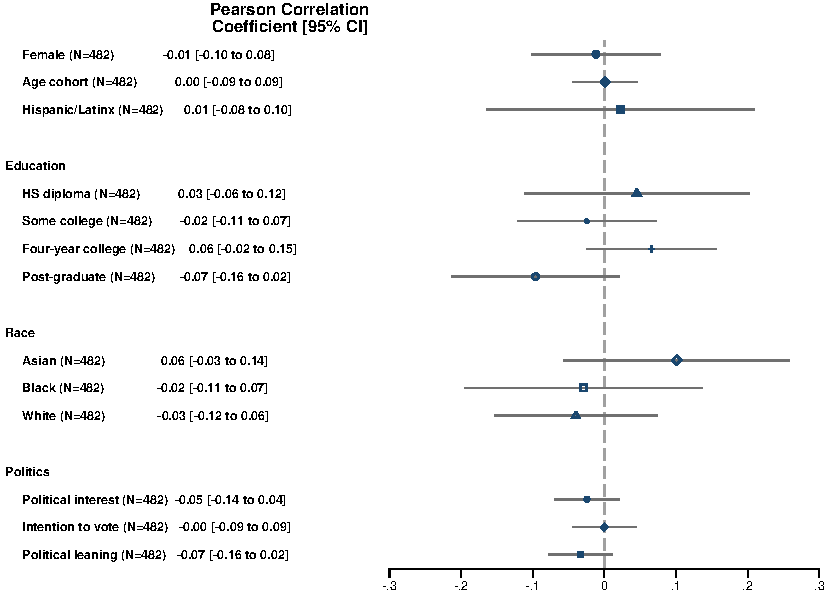
\includegraphics[scale=.8]{../figs/baltest-24k-rw.pdf}
  \label{fig:baltest-24k-rw}
  \caption*{\footnotesize Figure shows the results from a balance test for the Amazon Mechanical Turk sample. Self-reported characteristics of respondents are compared between the respondents assigned to the 24k arm and the RW arm as described in \nameref{sec:data}.
  Rows are self-reported characteristics.
  Second column reports the correlation between characteristics and the 24k arm, and the 95\% confidence intervals constructed from bootstrapped standard errors (n=10,000).
  Third column reports the estimated difference between the 24k respondents and the RW respondents.
  Horizontal bars are 95\% confidence intervals constructed from robust standard errors.
  }
\end{figure}
\end{center}
\fi

% MTurk Study 1 balance test: IDA vs CUD (IPS vs RW)
\begin{center}
	\begin{figure}[H]
		\centering
		\caption{MTurk Study 1---IDA and CUD}
		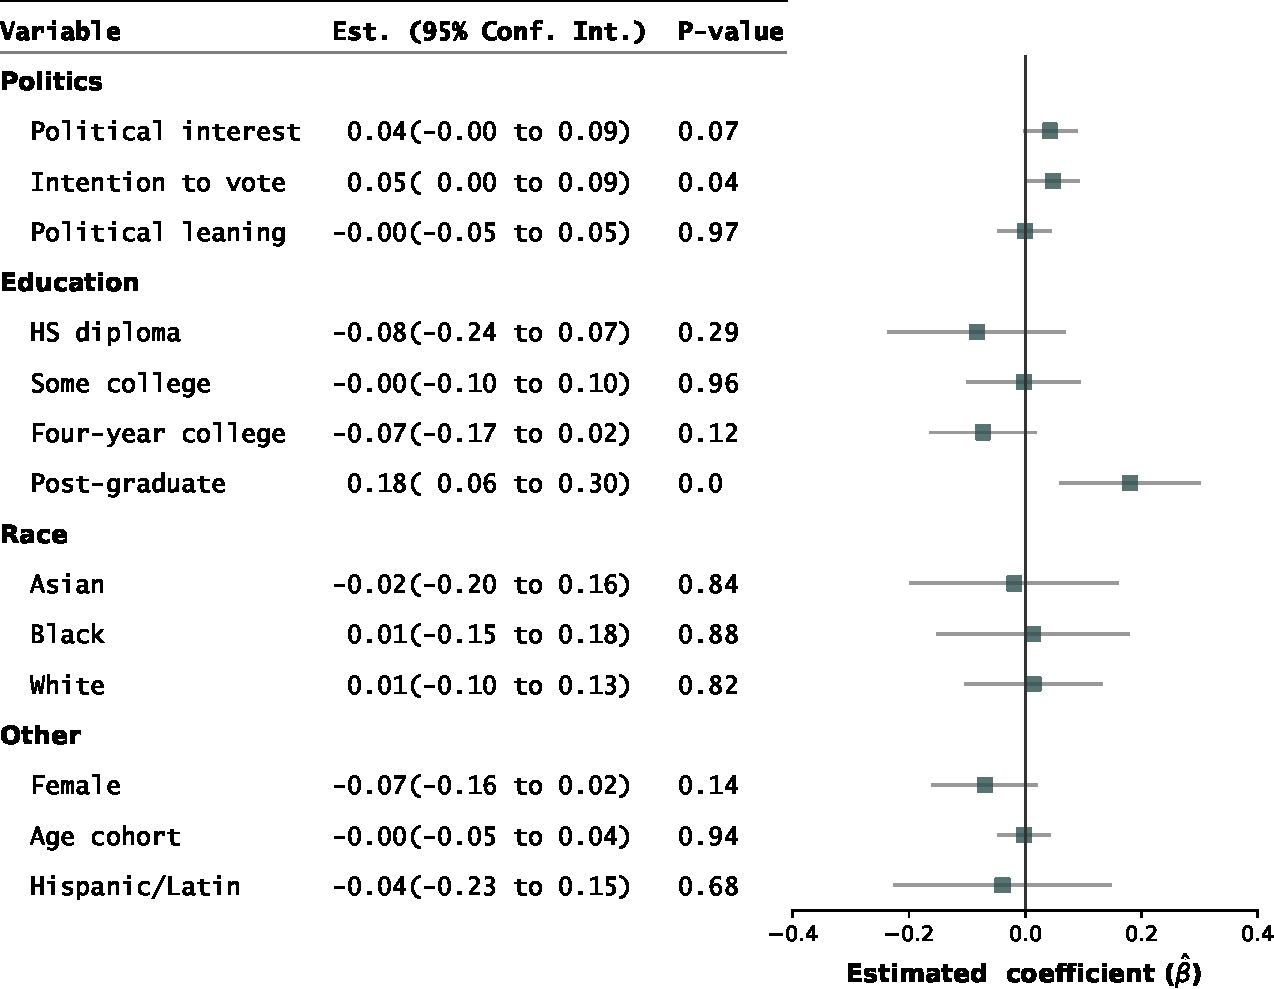
\includegraphics[width=\textwidth]{../figs/study1-baltest-RW-ips.pdf}
		\label{fig:baltest-24k-rw}
		\caption*{\footnotesize 
			Figure shows the balance tests of respondent characteristics for the Amazon Mechanical Turk Study 1 sample.
			The tests compares respondents assigned to the IDA condition vs. respondents assigned to the CUD condition.
			See \cref{tab:conditions} in \nameref{sec:inflationary_measures}.
			Rows are self-reported characteristics.
			Second column reports the estimates from regressing the characteristics on the CUD dummy, with IDA as the baseline.
			Third column reports the p-values.
			Horizontal bars are 95\% confidence intervals constructed from robust standard errors.
		}
	\end{figure}
\end{center}

% MTurk Study 1 balance test: IDA vs FSR (IPS vs FSR)
\begin{center}
	\begin{figure}
		\centering
		\caption{MTurk Study 1---IDA and FSR}
		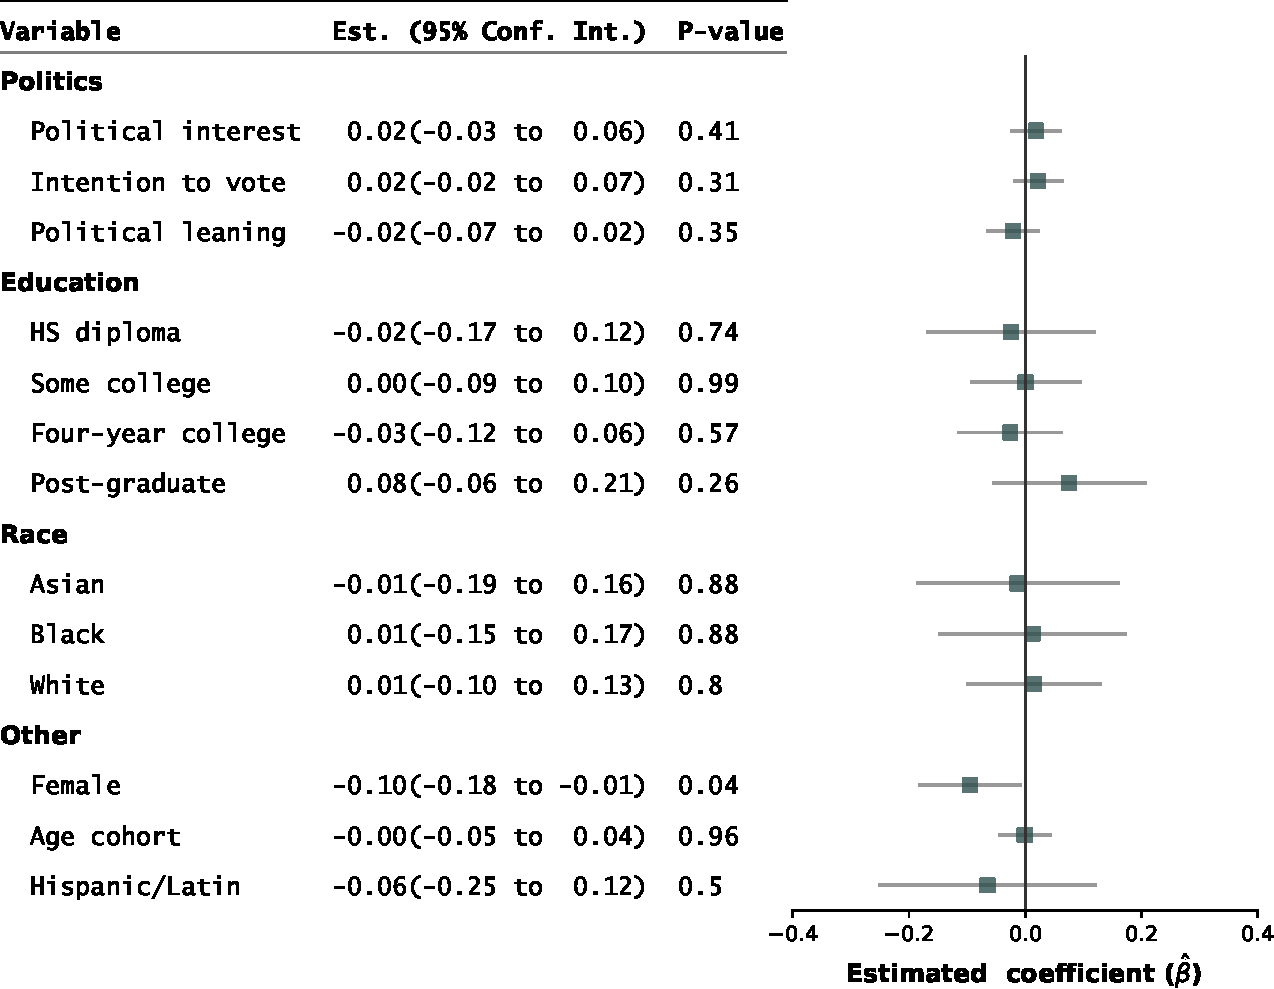
\includegraphics[width=\textwidth]{../figs/study1-baltest-FSR-ips.pdf}
		\label{fig:baltest-24k-rw}
		\caption*{\footnotesize 
			Figure shows the balance tests of respondent characteristics for the Amazon Mechanical Turk Study 1 sample.
			The tests compares respondents assigned to the IDA condition vs. respondents assigned to the FSR condition.
			See \cref{tab:conditions} in \nameref{sec:inflationary_measures}.
			Rows are self-reported characteristics.
			Second column reports the estimates from regressing the characteristics on the FSR dummy, with IDA as the baseline.
			Third column reports the p-values.
			Horizontal bars are 95\% confidence intervals constructed from robust standard errors.
		}
	\end{figure}
\end{center}

% MTurk Study 1 balance test: IDA vs IMC (IPS vs 14k)
\begin{center}
	\begin{figure}
		\centering
		\caption{MTurk Study 1---IDA and IMC}
		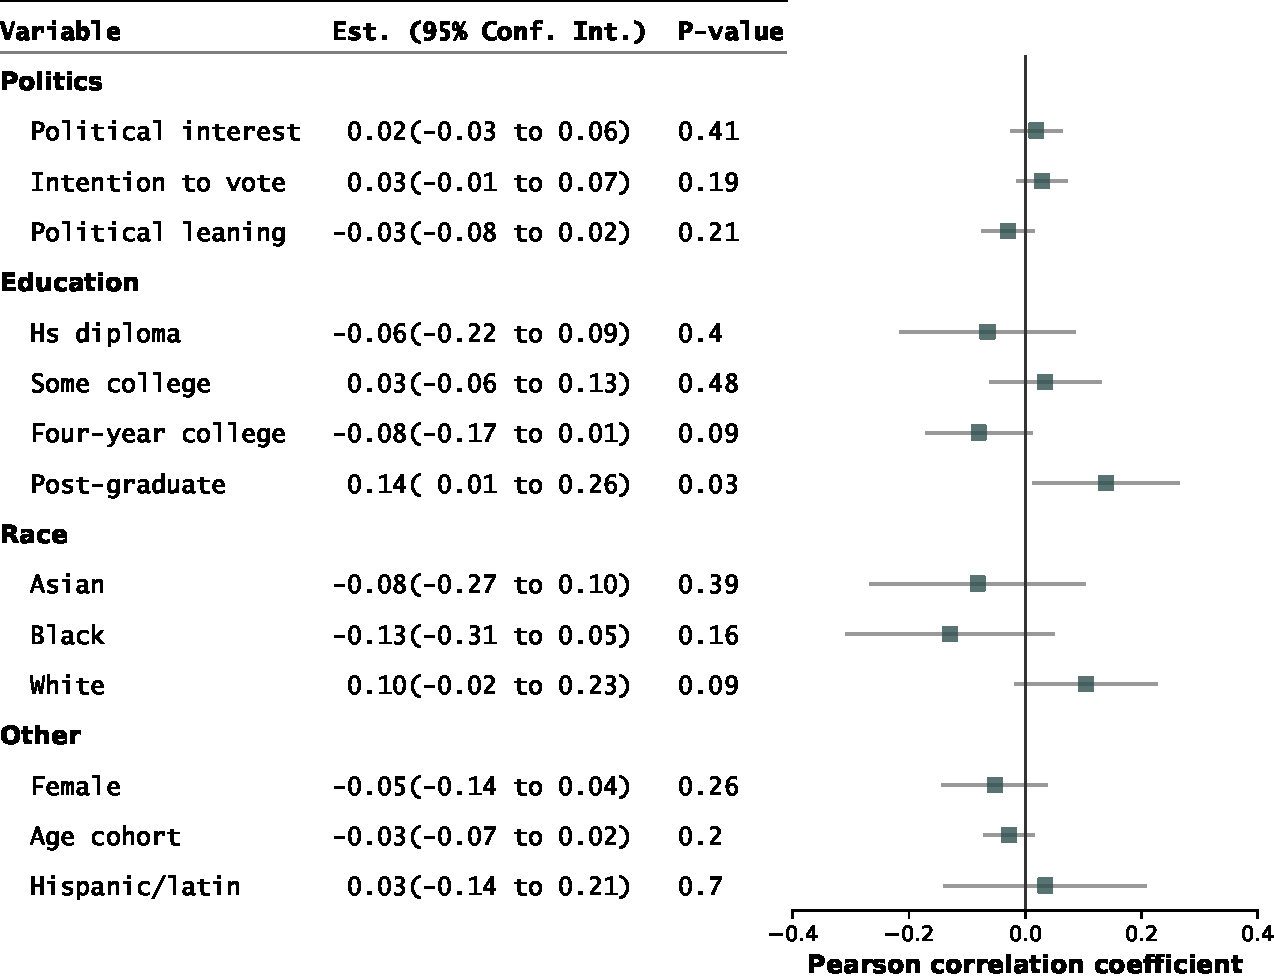
\includegraphics[width=\textwidth]{../figs/study1-baltest-14k-ips.pdf}
		\label{fig:baltest-24k-rw}
		\caption*{\footnotesize 
			Figure shows the balance tests of respondent characteristics for the Amazon Mechanical Turk Study 1 sample.
			The tests compares respondents assigned to the IDA condition vs. respondents assigned to the IMC condition.
			See \cref{tab:conditions} in \nameref{sec:inflationary_measures}.
			Rows are self-reported characteristics.
			Second column reports the estimates from regressing the characteristics on the IMC dummy, with IDA as the baseline.
			Third column reports the p-values.
			Horizontal bars are 95\% confidence intervals constructed from robust standard errors.
		}
	\end{figure}
\end{center}

% MTurk Study 1 balance test: IDA vs CCD (IPS vs 24k)
\begin{center}
	\begin{figure}
		\centering
		\caption{MTurk Study 1---IDA and CCD}
		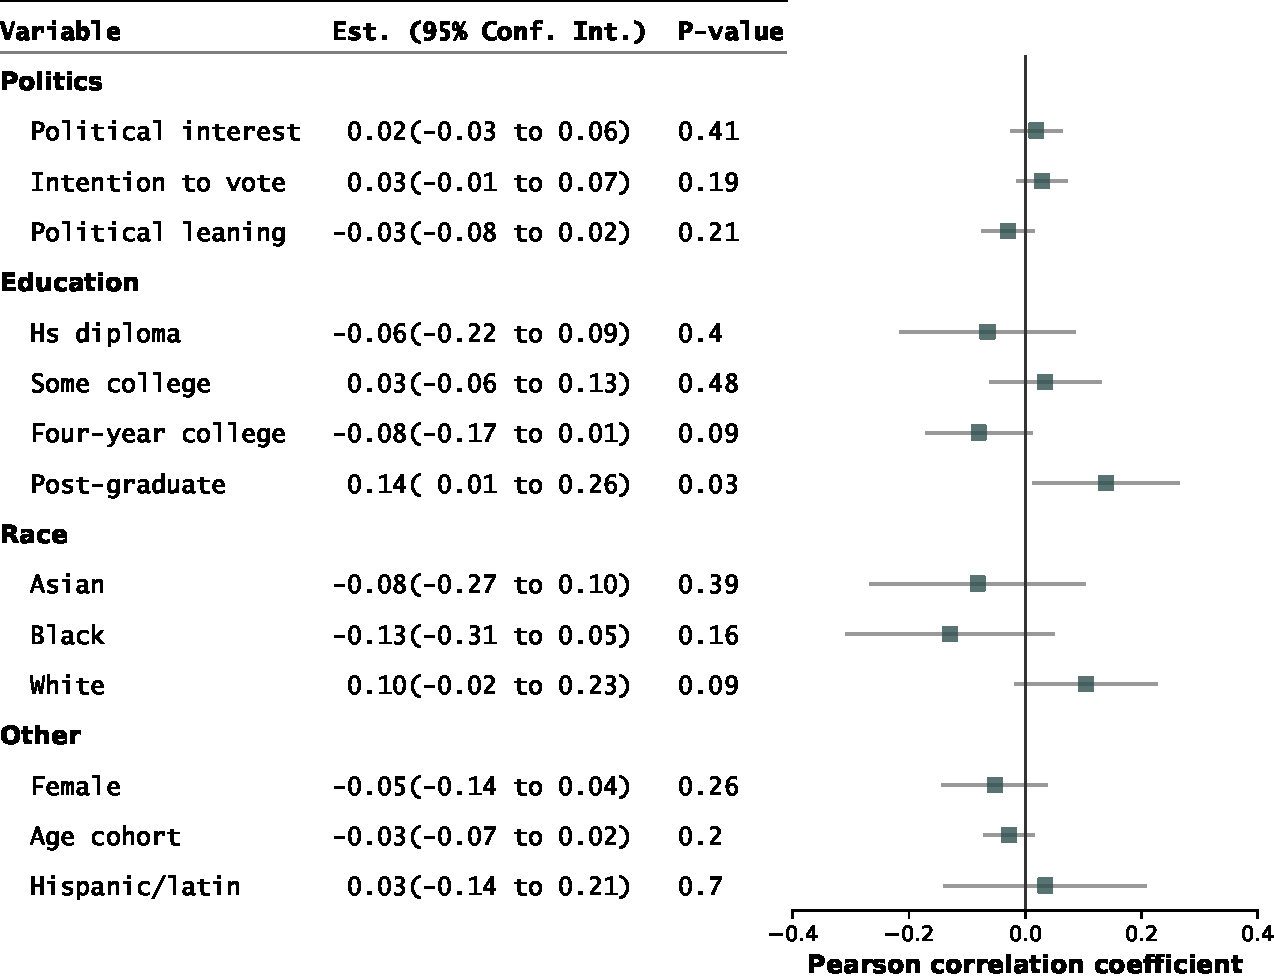
\includegraphics[width=\textwidth]{../figs/study1-baltest-14k-ips.pdf}
		\label{fig:baltest-24k-rw}
		\caption*{\footnotesize 
			Figure shows the balance tests of respondent characteristics for the Amazon Mechanical Turk Study 1 sample.
			The tests compares respondents assigned to the IDA condition vs. respondents assigned to the CCD condition.
			See \cref{tab:conditions} in \nameref{sec:inflationary_measures}.
			Rows are self-reported characteristics.
			Second column reports the estimates from regressing the characteristics on the CCD dummy, with IDA as the baseline.
			Third column reports the p-values.
			Horizontal bars are 95\% confidence intervals constructed from robust standard errors.
		}
	\end{figure}
\end{center}


\begin{figure}[ht]
	\caption{Partisan Knowledge Gaps with Partisan Cues: YouGov}
	\centering
	\begin{subfigure}{.495\textwidth}\centering
		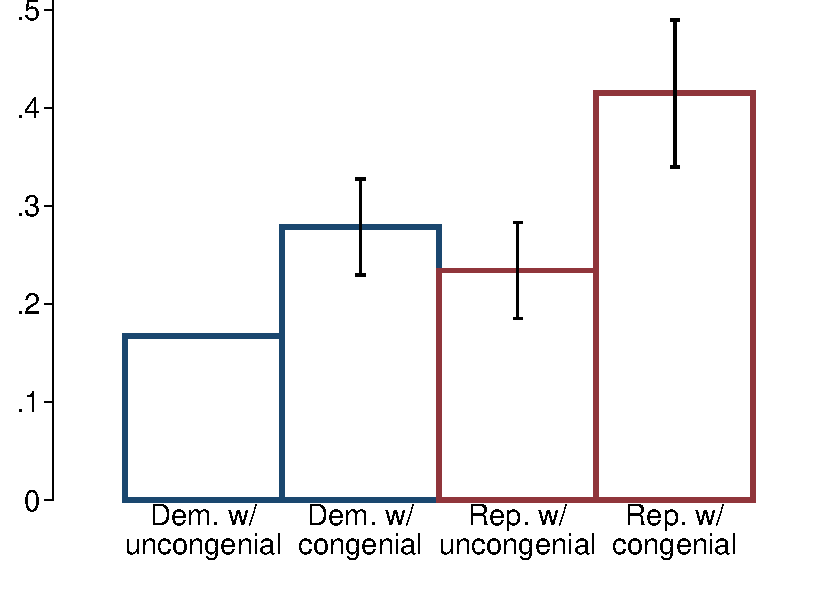
\includegraphics[width=\textwidth]{../figs/yougov-unemp-congenialcue-partisan.pdf}
		\caption{Unemployment}
	\end{subfigure}
	\hfil
	\begin{subfigure}{.495\textwidth}\centering
		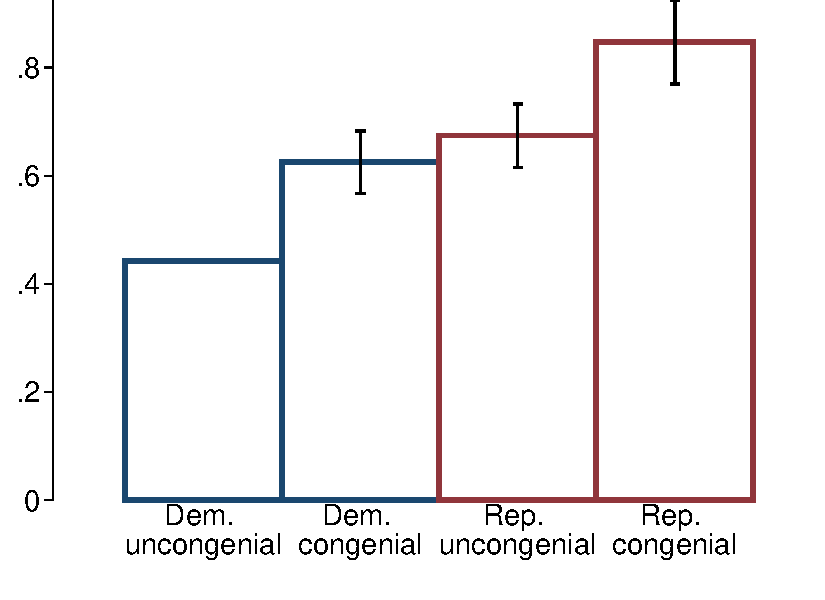
\includegraphics[width=\textwidth]{../figs/yougov-deficit-congenialcue-partisan.pdf}
		\caption{Budget deficit}
	\end{subfigure}
	\caption*{\footnotesize Figure shows the effect of congenial cues for the YouGov survey by partisanship. Bars indicate the predicted percent of responses saying that unemployment have gone up (correct response) as retrieved from the estimates in \cref{tab:partisangaps-yougov} (columns (2) and (5)).  The estimates are obtained by estimating:\\

	$\qquad\text{correct response}_{i} = \alpha + \beta (congenial \; cue)_i + \gamma (Rep)_i + \delta (congenial\; cue \times Rep)_i + \varepsilon_{i}$.\\

	Capped vertical bars indicate 95\% confidence intervals.
	}
	\label{fig:yougov-reg-by-partisanship}
\end{figure}

\clearpage
\section{Item Text for the MTurk Study}\label{si:mturk}

\textbf{Preface for Different Conditions}

\textbf{RW, IP}\newline
Now here are some questions about what you may know about politics and public affairs.

\textbf{FSR, 14k, 24k}\newline
Now here are some questions about what you may know about politics and public affairs.
We are interested in measuring what people currently know and can recall on their own and are
just as interested in what people don't know as in what they do know. So we'd like your
agreement to just say ``don't know'' if you don't know the answer—without looking anything up
or talking with anyone about it.

\textbf{Item Text}
\textbf{24k}\newline
Now here are a series of statements. On a scale of 0 to 10, where 0 means definitely false,
10 means definitely true, and 5 is exactly in the middle, how definitely true or false is
each statement?

\begin{itemize}
	\item Barack Obama was born in the US (T)
	\item  Barack Obama is a Muslim (F)
	\item  The Affordable Care Act gives illegal immigrants financial help to buy health insurance (F)
	\item  The Affordable Care Act does not create government panels to make decisions about end-of-life care (T)
	\item  Temperatures around the world are increasing because of human activity, like burning coal and gasoline (T)
	\item  Most climate scientists believe that global warming is not occurring (F)
	\item  In the 2016 presidential election, President Trump won the majority of the legally cast votes (F)
	\item  The vaccine for measles, mumps, and rubella (MMR) causes autism in children. (F)
	\item  Since 2012, the annual federal budget deficit has increased. (T)
\end{itemize}

\textbf{Rest of the Conditions, By Item}

\begin{itemize}
\item Obama's Birthplace

\textbf{RW and IP}\newline

According to the Constitution, American presidents must be ``natural born citizens.''
Some people believe Barack Obama was not born in the United States, but was born
in another country. Do you think Barack Obama was born in ...?
\begin{itemize}
	\item The US
	\item Another country
\end{itemize}

\textbf{FSR}\newline
Some people believe Barack Obama was not born in the United States, but was born
in another country. Was he born in ...?
\begin{itemize}
	\item The US
	\item Another country
	\item DK (plus DK pref)
\end{itemize}

\textbf{14k}\newline

Was Barack Obama born in ...?
\begin{itemize}
	\item the US
	\item Another country
	\item DK (plus DK pref)
\end{itemize}

\item Obama Religion\newline
\textbf{RW}\newline

Do you personally believe that Barack Obama is a ...?
\begin{itemize}
	\item Muslim
	\item Christian
\end{itemize}

\textbf{IP}\newline

Most people have a religion. Some people believe Barack Obama is a Muslim. Do
you personally believe that Barack Obama is a \ldots?
\begin{itemize}
	\item Muslim
	\item Christian
\end{itemize}

\textbf{FSR}\newline

Some people believe Barack Obama is a Muslim. Is he a \ldots?
\begin{itemize}
	\item Muslim
	\item Christian
	\item DK (+ DK pref)
\end{itemize}

\textbf{14k}\newline

Is Barack Obama a \ldots?
\begin{itemize}
	\item Muslim
	\item Christian
	\item DK (plus DK pref)
\end{itemize}

\item ACA Illegal\newline
\textbf{RW}\newline

To the best of your knowledge, would you say the Affordable Care Act\ldots?
\begin{itemize}
	\item Gives illegal immigrants financial help to buy health insurance
	\item Does not give illegal immigrants financial help to buy health insurance
\end{itemize}

\textbf{IP}\newline

As you may know, there is currently talk of changing the Affordable Care Act
(ACA), enacted in 2010. Some people believe that the ACA gives illegal immigrants
financial help to buy health insurance. To the best of your knowledge, would you say
the ACA\ldots?
\begin{itemize}
	\item Gives illegal immigrants financial help to buy health insurance
	\item Does not give illegal immigrants financial help to buy health insurance
\end{itemize}

\textbf{FSR}\newline

Some people believe that Affordable Care Act gives illegal immigrants financial help
to buy health insurance. Does the Affordable Care Act\ldots?
\begin{itemize}
	\item Give illegal immigrants financial help to buy health insurance
	\item Not give illegal immigrants financial help to buy health insurance
	\item DK (+ DK pref)
\end{itemize}

\textbf{14k}\newline
Does the Affordable Care Act\ldots?
\begin{itemize}
	\item Give illegal immigrants financial help to buy health insurance
	\item Not Give illegal immigrants financial help to buy health insurance
	\item Don't know (+ DK pref)
\end{itemize}

\item ACA—Death Panels\newline
\textbf{RW}\newline
To the best of your knowledge, would you say that the Affordable Care Act \ldots?
\begin{itemize}
	\item Creates government panels to make decisions about end-of-life care
	\item Does not create government panels to make decisions about end-of-life care
\end{itemize}

\textbf{IP}\newline

Some people believe that Affordable Care Act establishes a government panel to
make decisions about end-of-life care. To the best of your knowledge, would you say
that the Affordable Care Act \ldots?
\begin{itemize}
	\item Creates government panels to make decisions about end-of-life care
	\item Does not create government panels to make decisions about end-of-life care
\end{itemize}

\textbf{FSR}\newline

Some people believe that Affordable Care Act establishes a government panel to
make decisions about end-of-life care. Does the Affordable Care Act\ldots?
\begin{itemize}
	\item Creates government panels to make decisions about end-of-life care
	\item Does not create government panels to make decisions about end-of-life care
	\item DK (+ DK pref)
\end{itemize}

\textbf{14k}\newline
Does the Affordable Care Act \ldots?
\begin{itemize}
	\item Creates government panels to make decisions about end-of-life care
	\item Does not create government panels to make decisions about end-of-life care
	\item DK (+ DK pref)
\end{itemize}

\item Global Warming—Happening + Causes\newline
\textbf{RW}\newline
Which of the following best fits your view about this? Are temperatures around the
world \ldots?
\begin{itemize}
	\item Increasing because of natural variation over time, such as produced the ice age
	\item Increasing because of human activity, like burning coal and gasoline
	\item Staying about the same as they have been
\end{itemize}

\textbf{IP}\newline
Recently, you may have noticed that global warming has been getting some attention
in the news. Some people believe that temperatures are increasing around the world
because of natural variation over time, such as produced the ice age. Which of the
following best fits your view about this? Would you say that temperatures around the
world are\ldots?
\begin{itemize}
	\item Increasing because of natural variation over time, such as produced the ice age
	\item Increasing because of human activity, like burning coal and gasoline
	\item Staying about the same as they have been
\end{itemize}

\textbf{FSR}\newline

Some people believe that temperatures are increasing around the world because of
natural variation over time, such as produced the ice age. Are temperatures around
the world \ldots?
\begin{itemize}
	\item Increasing because of natural variation over time, such as produced the ice age
	\item Increasing because of human activity, like burning coal and gasoline
	\item Staying about the same as they have been
	\item DK (+ DK pref)
\end{itemize}

\textbf{14k}\newline
Are temperatures around the world \ldots?
\begin{itemize}
	\item Increasing because natural variation over time, such as produced the ice age
	\item Increasing because human activity, like burning coal and gasoline
	\item Staying about the same as they have been
	\item DK (+ DK pref)
\end{itemize}

\item GW—Scientist Agreement\newline
\textbf{RW}\newline
Just your impression, which one of the following statements do you think is most
accurate?
\begin{itemize}
	\item Most climate scientists believe that global warming is occurring.
	\item Most climate scientists believe that global warming is not occurring.
	\item Climate scientists are about equally divided about whether global warming is occurring or not
\end{itemize}

\textbf{IP}\newline
As you may know, the term ``global warming'' refers to the claim that temperatures
have been increasing around the world. Some people believe that most climate
scientists believe that global warming is not occurring. Just your impression, which
one of the following statements do you think is most accurate?
\begin{itemize}
	\item Most climate scientists believe that global warming is occurring.
	\item Most climate scientists believe that global warming is not occurring.
	\item Climate scientists are about equally divided about whether global warming is occurring or not
\end{itemize}
\textbf{FSR}\newline
Some people believe that most climate scientists believe that global warming is not
occurring. Which one of the following statements is most accurate?
\begin{itemize}
	\item Most climate scientists believe that global warming is occurring.
	\item Most climate scientists believe that global warming is not occurring.
	\item Climate scientists are about equally divided about whether global warming is occurring or not
	\item DK (+ DK pref)
\end{itemize}

\textbf{14k}\newline
Which one of the following statements is most accurate?
\begin{itemize}
	\item Most climate scientists believe that global warming is occurring.
	\item Most climate scientists believe that global warming is NOT occurring.
	\item Climate scientists are about equally divided about whether global warming is occurring or not
	\item DK (+ DK pref)
\end{itemize}

\item Voter Fraud\newline
\textbf{RW}\newline
As you may know, President Trump has said that several million people voted
illegally in the 2016 presidential election and that he won the majority of the legally
cast votes. Do you believe that President Trump \ldots?
\begin{itemize}
	\item Won the majority of the legally cast votes
	\item Did not win the majority of the legally cast votes
\end{itemize}

\textbf{IP}\newline
As you may know, not everyone living in the US has the legal right to vote. President
Trump has said that several million people voted illegally in the 2016 presidential
election and that he won the majority of the legally cast votes. Do think that that
President Trump \ldots?
\begin{itemize}
	\item Won the majority of the legally cast votes
	\item Did not win the majority of the legally cast votes
\end{itemize}

\textbf{FSR}\newline
As you may know, President Trump has said that several million people voted
illegally in the 2016 presidential election and that he won the majority of the legally
cast votes. Did President Trump \ldots?
\begin{itemize}
	\item Won the majority of the legally cast votes
	\item Did not win the majority of the legally cast votes
	\item DK (+ DK pref)
\end{itemize}

\textbf{14k}\newline
In the 2016 presidential election, did President Trump \ldots?
\begin{itemize}
	\item Won the majority of the legally cast votes
	\item Did not win the majority of the legally cast votes
	\item DK (+ DK pref)
\end{itemize}

\item Vaccines\newline
\textbf{RW}\newline
From what you have read or heard, do you personally think that the vaccine for
Measles, Mumps, and Rubella (MMR):
\begin{itemize}
	\item Causes autism in children
	\item Does not cause autism is children
\end{itemize}

\textbf{IP}\newline
As you may know, most children receive the vaccine for Measles, Mumps, and
Rubella (MMR). Some people believe that the MMR vaccine causes autism in
children. From what you have read or heard, do you personally think that the MMR
vaccine:
\begin{itemize}
	\item Causes autism in children
	\item Does not cause autism is children
\end{itemize}

\textbf{FSR}\newline
Some people believe that the vaccine for Measles, Mumps, and Rubella (MMR)
causes autism in children. Does the MMR vaccine \ldots?
\begin{itemize}
	\item Cause autism in children
	\item Not cause autism in children.
	\item DK (+ DK pref)
\end{itemize}

\textbf{14k}\newline
Does the vaccine for Measles, Mumps, and Rubella (MMR) \ldots?
\begin{itemize}
	\item Cause autism in children
	\item Not cause autism in children.
	\item DK (+ DK pref)
\end{itemize}

\item Obama—Budget Deficit\newline
\textbf{RW}\newline
As you may know, the federal government runs a deficit when it spends more than it
takes in. Since 2012, would you say that the annual federal budget deficit has \ldots
\begin{itemize}
	\item Increased
	\item Stayed about the same
	\item Decreased
\end{itemize}

\textbf{IP}\newline
As you may know, the federal government runs a deficit when it spends more than it
takes in. Since 2012, with the Republicans having the majority in the U.S. House of
Representatives, would you say that the annual federal budget deficit has \ldots
\begin{itemize}
	\item Increased
	\item Stayed about the same
	\item Decreased
\end{itemize}

\textbf{FSR}\newline
Since 2012, with the Republicans having the majority in the U.S. House of
Representatives,
\begin{itemize}
	\item has the annual federal budget deficit \ldots.
	\item Increased
	\item Stayed about the same
	\item Decreased
	\item DK (+ DK pref)
\end{itemize}

\textbf{14k}\newline

Since 2012, has the annual federal budget deficit \ldots
\begin{itemize}
	\item Increased
	\item Stayed about the same
	\item Decreased
	\item DK (+ DK pref)
\end{itemize}
\end{itemize}

\newpage




\clearpage
\section{Item Text for the Second MTurk Study}\label{si:mturk2}


The second Amazon MTurk survey was fielded in April 2017 and had 1,059 participants. In this survey we made use of new questions and probes to examine the effect of question design on (partisan) knowledge. We asked the participants four questions about the Affordable Care Act (2), the effect of greenhouse gases (1), and Donald Trump's recent executive order on immigration (1).

\begin{comment}
\noindent
\textbf{Rules for Coding Open Ended Questions}\newline

In coding open-ended responses, all misspellings, modifications, synonyms, and identifiable abbreviations of a word were fully credited.


\noindent
\textbf{Honesty Pledge}

At the beginning of the survey, a random two-thirds of the respondents were asked to commit to not look up the answers or to ask anyone about the answers. Rest one-third of the participants didn’t see any message at the start.


\noindent
\textbf{Photo Vs. Text}

Individuals were asked knowledge questions about domestic and international political leaders. These leaders were presented to the participants either as a photo (asking for name or position) or they saw the name as text (asking for the position).

\noindent
The preamble for the two treatments were:

\begin{description}
\item[Photo:] Here’s a set of photos. For each photo, can you tell me what position he or she holds? If you don’t know, don’t worry about it. Just leave the space blank, and move on to the next person. What position does this person hold?
  \item[Text:] Here’s a list of names. For each name, can you tell me what position that person holds? If you don’t know, don’t worry about it. Just leave the space blank, and move on to the next person. What position does this person hold?
\end{description}


\begin{itemize}
\item Mitch McConnell
  \begin{itemize}
\item  OE: (Senate OR majority) AND (leader OR chief OR head OR president OR chair OR whip)
\end{itemize}
\item Chuck Schumer
  \begin{itemize}
\item  OE: (Senate OR minority) AND (leader OR in charge)
\end{itemize}
\item Angela Merkel
    \begin{itemize}
\item OE: German AND (President OR Leader OR Prime Minister OR Chancellor OR Premier AND Ruler AND charge)
\end{itemize}
\item Vladimir Putin
  \begin{itemize}
\item OE: Russia AND (President OR Leader OR Head OR Chancellor OR Premier OR Prime Minister)
\end{itemize}
\item John Roberts
  \begin{itemize}
\item OE: Chief AND Justice
\end{itemize}
\item Nancy Pelosi
  \begin{itemize}
\item OE: Minority AND Leade
\end{itemize}
\end{itemize}

\end{comment}

One half of the survey respondents got a conventional closed-ended item with five options including the opportunity to mark Don’t know. The other half of the respondents had to assess the truth of statements on a scale from definitely false (0) to definitely true (10).


\begin{description}
\item[1.] Does the Affordable Care Act ...?
  \begin{itemize}
    \item  CE: Provide coverage for people who are currently in the country illegally, Replace private health insurance with a ``single payer system'', \textbf{Increase the Medicare payroll tax for upper-income Americans}, Reimburse routine mammograms only for women older than 50, Don’t know (5)
    \item  Scale: Rating each response option above from definitely false (0) to definitely true (10). Don’t know was not included. See Figure \ref{fig:aca1}.
    \end{itemize}
    \item[2.] Are greenhouse gases ...?
  \begin{itemize}
  \item CE: A cause of respiratory problems, A cause of for lung cancer, Damaging the ozone layer, \textbf{A cause of rising sea levels}, or Don’t know
  \item Scale: Rating each response option above from definitely false (0) to definitely true (10). Don’t know was not included. See Figure \ref{fig:gg1}.
    \end{itemize}
  \item[3.] And does the Affordable Care Act ...?
    \begin{itemize}
  \item CE: Create government panels to make end-of-life decisions for people on Medicare, Replace Medicare with a ``public option'', \textbf{Limit future increases in payments to Medicare providers}, Cut benefits to existing Medicare patients, Don’t know
  \item Scale: Rating each response option above from definitely false (0) to definitely true (10). Don’t know was not included. See Figure \ref{fig:aca2}.
    \end{itemize}
        \item[4.] Does President Trump’s most recent executive order on immigration ...?
  \begin{itemize}
  \item  CE: Subject immigrants living in the U.S. illegally to deportation, Strip immigrants from countries supporting terrorism of their green cards, Strip immigrants from several Muslim-majority countries of their green cards, \textbf{Temporarily ban immigrants from several majority-Muslim countries}, Don’t know
    \item  Scale: Rating each response option above from definitely false (0) to definitely true (10). Don’t know was not included. See Figure \ref{fig:eo1}.
    \end{itemize}
    \end{description}

If the close-ended questions 3 and 4 were not answered with Don’t know the respondents received one of two a follow- up question:
\begin{itemize}
\item OE: What made you choose that response?
 \item CE: What made you choose that response? I asked someone I know, I looked it up, I’ve read, seen, or heard that, It makes me feel good to think that, It makes sense, in view of other things I know, I just thought I’d take a shot
\end{itemize}

\begin{center}
	\begin{figure}[H]
		\centering
		\caption{Affordable Care Act 1 Scale Question}
		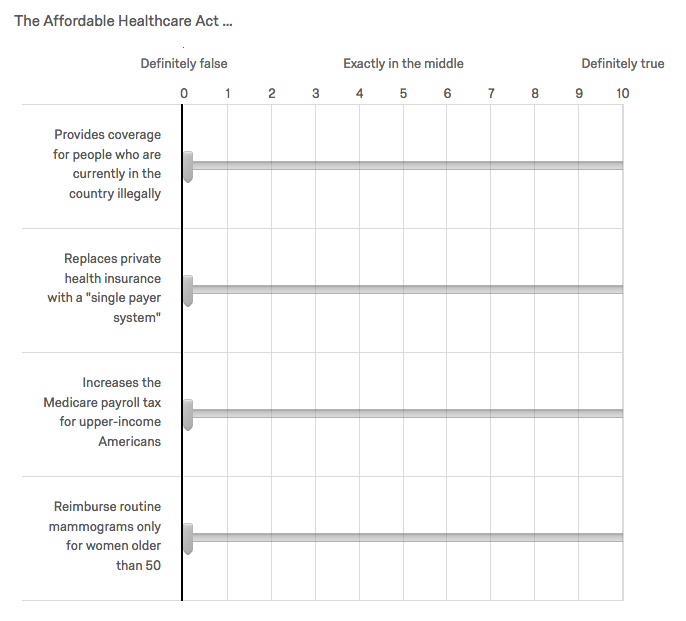
\includegraphics[width=\textwidth]{../figs/hk_aca1.png}
		\label{fig:aca1}
		\caption*{\footnotesize }
	\end{figure}
\end{center}


\begin{center}
	\begin{figure}[H]
		\centering
		\caption{Greenhouse Gases Scale Question}
		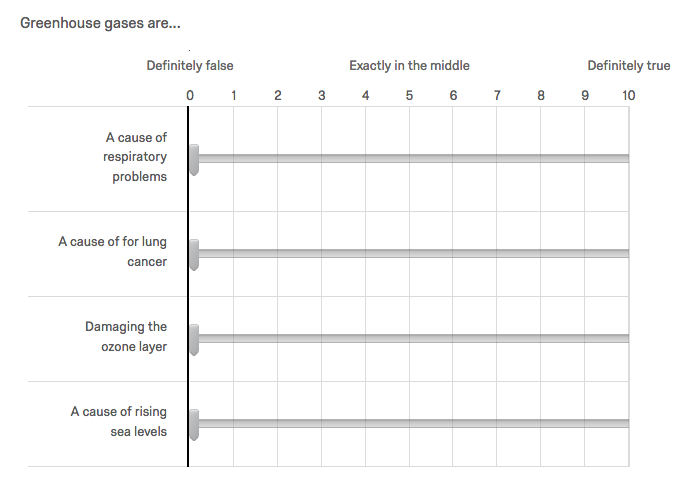
\includegraphics[width=\textwidth]{../figs/hk_gg1.png}
		\label{fig:gg1}
		\caption*{\footnotesize }
	\end{figure}
\end{center}


\begin{center}
	\begin{figure}[H]
		\centering
		\caption{Affordable Care Act 2 Scale Question}
		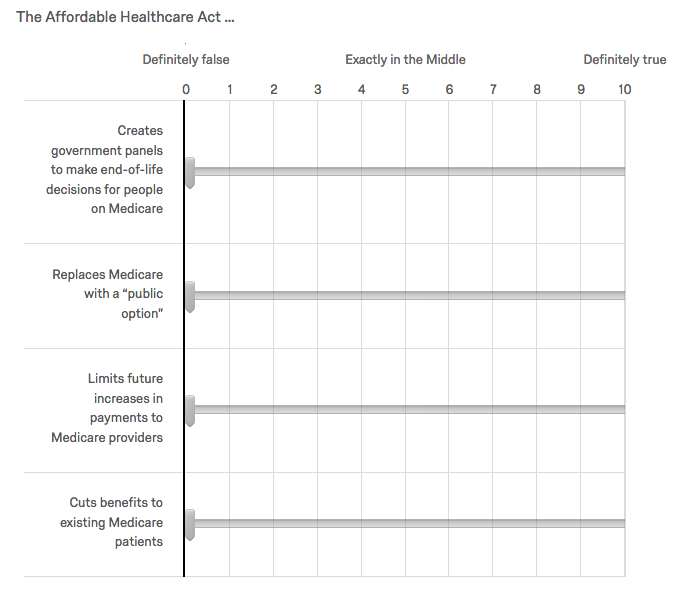
\includegraphics[width=\textwidth]{../figs/hk_aca2.png}
		\label{fig:aca2}
		\caption*{\footnotesize }
	\end{figure}
\end{center}


\begin{center}
	\begin{figure}[H]
		\centering
		\caption{Executive Order Scale Question}
		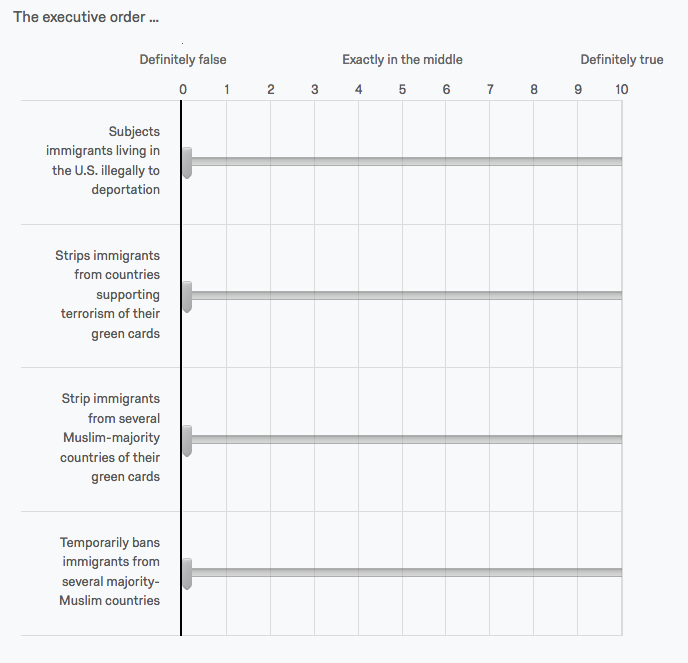
\includegraphics[width=\textwidth]{../figs/hk_eo1.png}
		\label{fig:eo1}
		\caption*{\footnotesize }
	\end{figure}
\end{center}

\newpage

\noindent
\textbf{Inference}

The following close-ended two deficit related questions were presented to all survey participants.

\begin{enumerate}
    \item During the time Barack Obama was president, the federal deficit: \textbf{Increased}, Remained about the same, Decreased, Don’t Know
    \item During the time George W. Bush was president, the federal deficit: \textbf{Increased}, Remained about the same, Decreased, Don’t Know
\end{enumerate}

Both questions were followed by a probe. For one half of the respondents this probe was open and for the other one the probe was closed.
\begin{itemize}
 \item OE: What made you choose that response?
 \item CE: What made you choose that response? I asked someone I know, I looked it up, I’ve read, seen, or heard that, It makes me feel good to think that, It makes sense, in view of other things I know, I just thought I’d take a shot
\end{itemize}



\end{document}